% preamble with all definitions
\documentclass[12pt,letterpaper]{book}
\usepackage{graphicx}
\usepackage{fancyhdr}  
\usepackage{amsmath, amsthm, amssymb}
\usepackage{booktabs}
\usepackage{subfig}
\usepackage{pdfpages}
\usepackage{braket}
\usepackage{pdflscape}
\usepackage{longtable}
\usepackage{enumerate}
\usepackage{pdfpages}
\usepackage[ngerman,english]{babel}
%\usepackage[left=2.0cm,right=2.0cm,top=2cm,bottom=2cm]{geometry}
\usepackage[utf8]{inputenc}
\usepackage{amsmath}
\usepackage{amsfonts}
\usepackage{amssymb}
\usepackage{fancybox}
\usepackage{xcolor}
\usepackage{listings}
\lstset{
  mathescape = true,
  basicstyle = \ttfamily}
\newcommand{\dollar}{\mbox{\textdollar}}
\usepackage{fancyvrb}

%% title page with background
\usepackage[pages=some]{background}
\backgroundsetup{scale = 1, angle = 0, opacity = 0.95,
  contents = {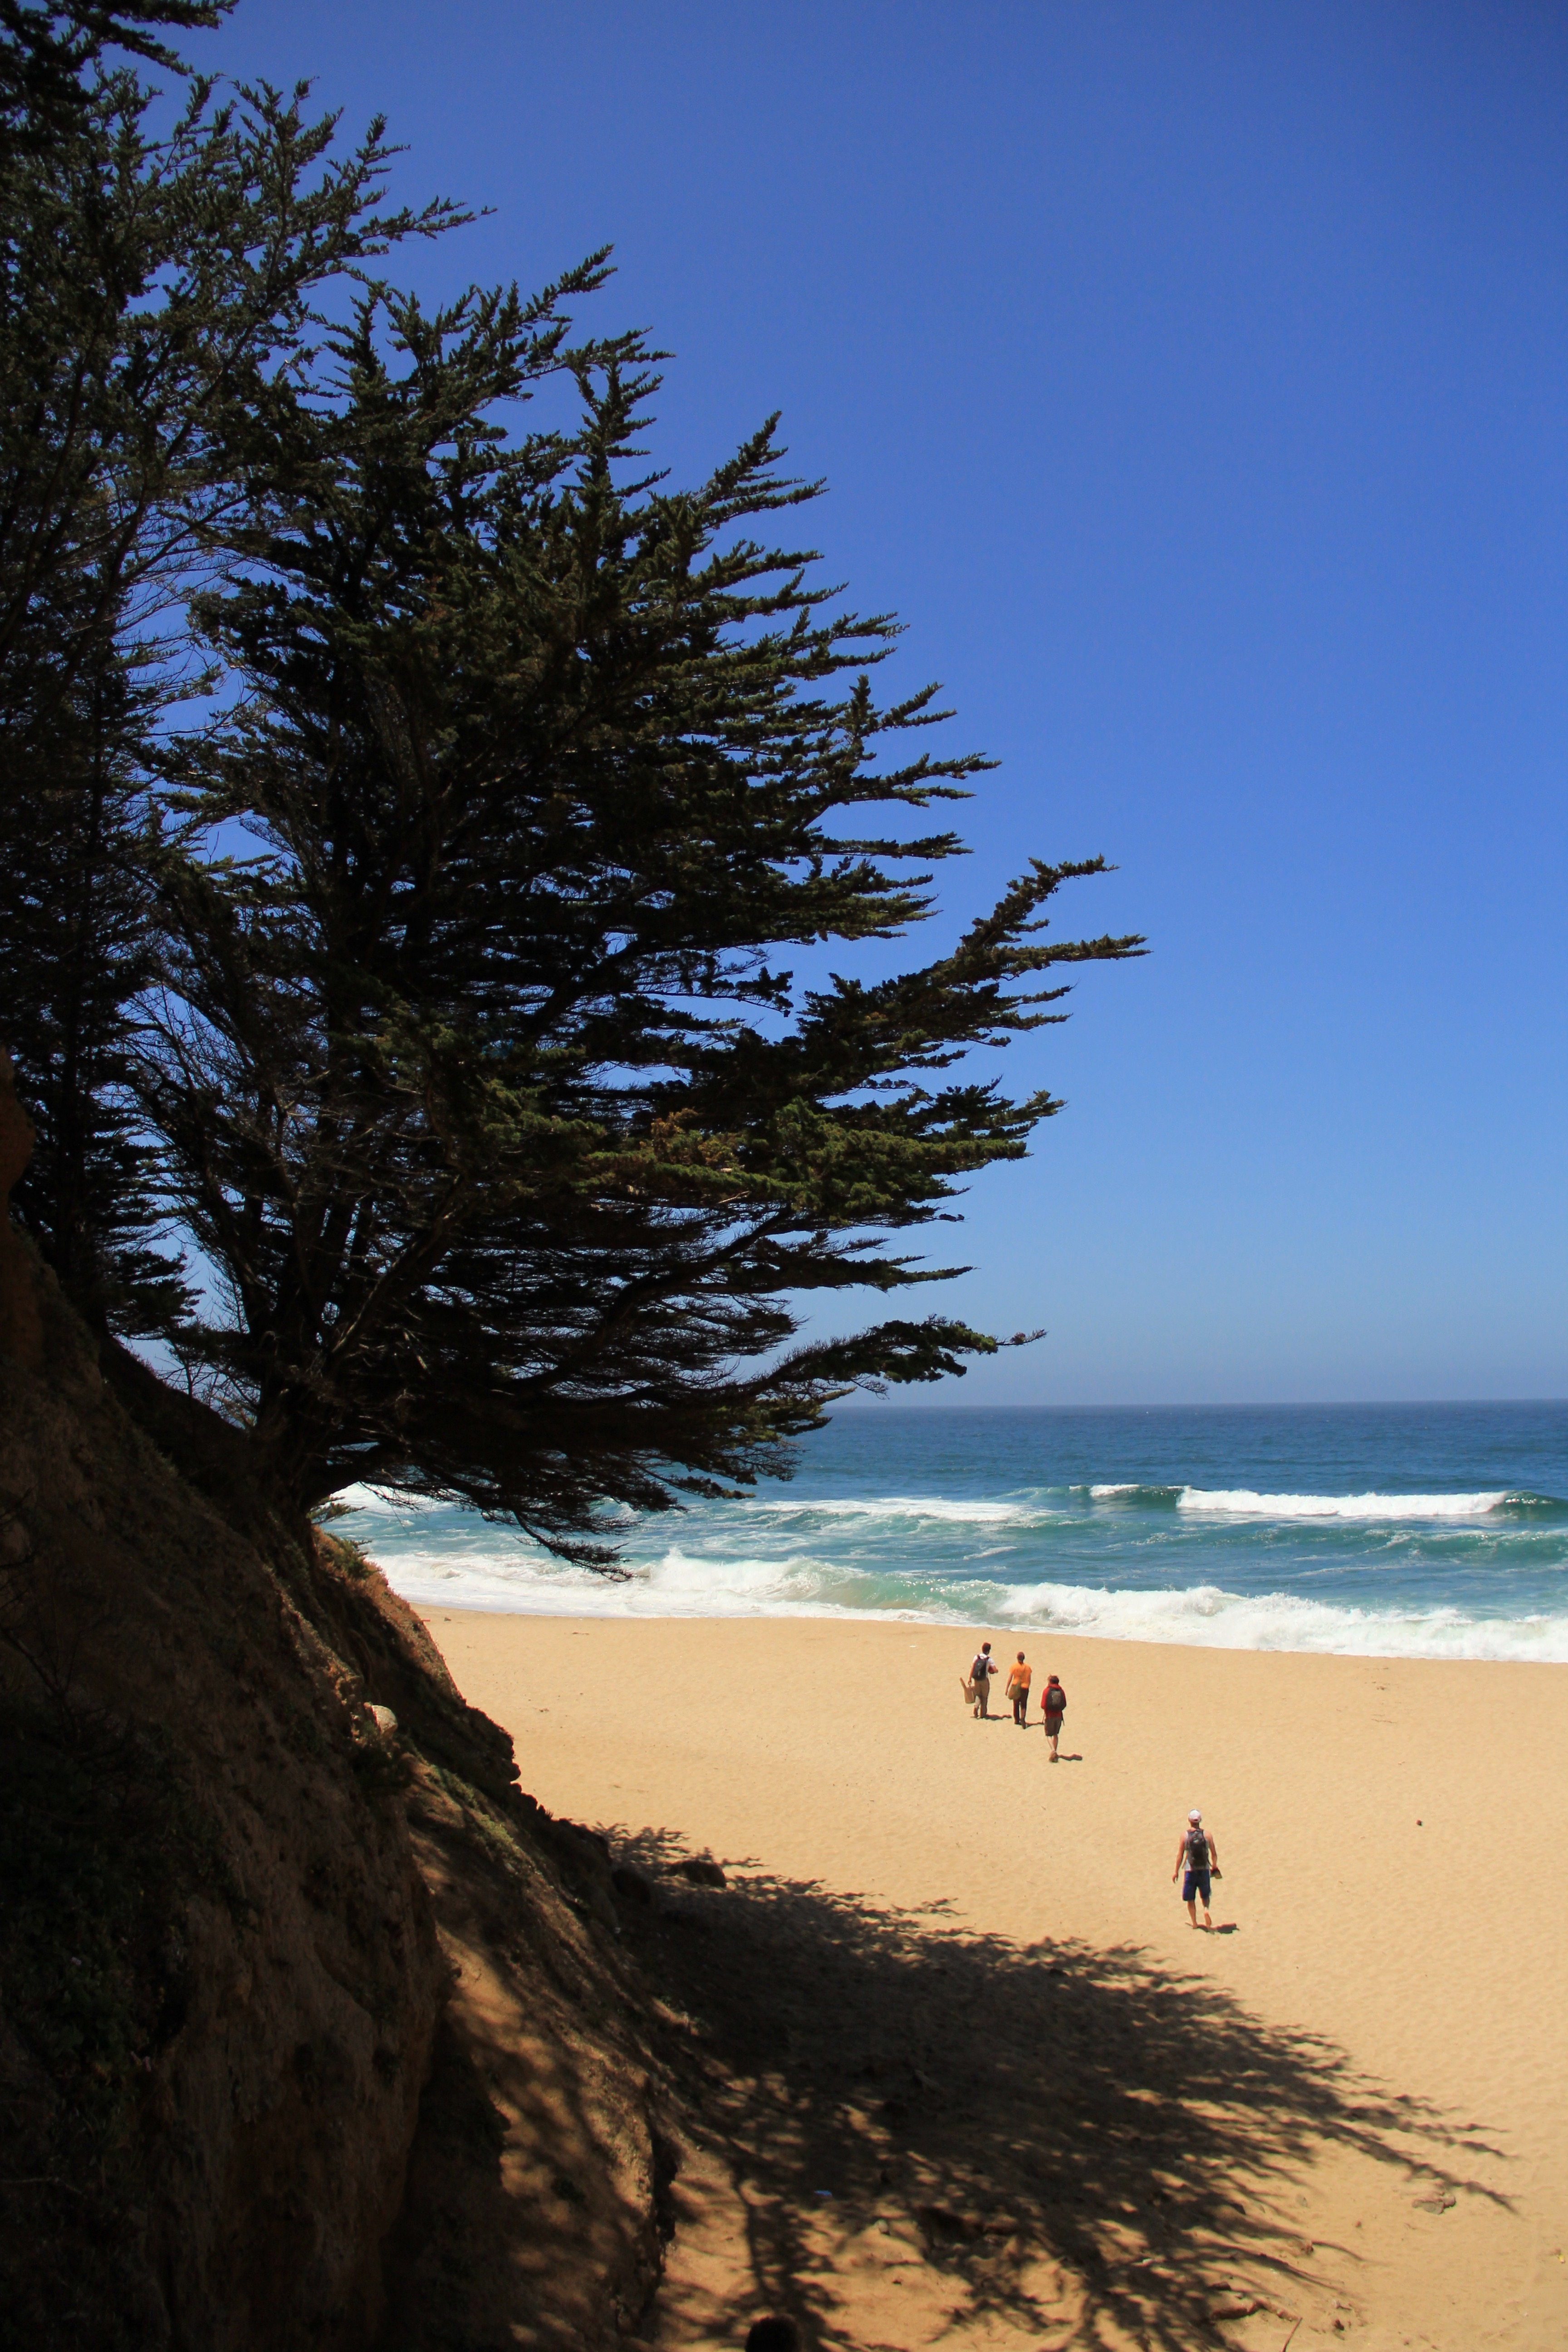
\includegraphics[width = 1.0\paperwidth,
    height = 1.0\paperheight, keepaspectratio]
      {pics/IMG_7946.jpg}}}
        % Adjust filename and path to match your own image 

%%%%%%%Some style changes
\addtolength\textwidth{25mm}
\addtolength\textheight{40mm}
\addtolength\voffset{-20mm}
%\addtolength\oddsidemargin{10mm}
\addtolength\evensidemargin{-20mm}
\usepackage{caption}
\setlength{\captionmargin}{10mm}
\renewcommand\captionfont{\it}
\renewcommand\captionlabelfont{\bf}

\newcommand{\fref}[1]{Figure~\ref{#1}}
\newcommand{\tref}[1]{Table~\ref{#1}}
\newcommand{\tsref}[1]{Tables~\ref{#1}}
\newcommand{\eref}[1]{Equation~\ref{#1}}
\newcommand{\esref}[1]{Equations~\ref{#1}}
\newcommand{\cref}[1]{Chapter~\ref{#1}}
\newcommand{\sref}[1]{Section~\ref{#1}}
\newcommand{\aref}[1]{Appendix~\ref{#1}}
\newcommand{\vecop}[1]{\mathbf{\hat{#1}}}
\newcommand{\op}[1]{\hat{#1}}
\newcommand{\Mu}[0]{\mathrm{Mu}}
\newcommand{\Ref}[0]{\mathrm{ref}}
\newcommand{\tot}[0]{\mathrm{tot}}
\newcommand{\res}[0]{\mathrm{res}}
\newcommand{\In}[0]{\mathrm{in}}
\newcommand{\ud}[0]{\mathrm{ud}}
\newcommand{\out}[0]{\mathrm{out}}
\newcommand{\corr}[0]{\mathrm{corr}}
\newcommand{\quartz}[0]{\mathrm{quartz}}
\newcommand{\fsample}[0]{\mathrm{F}}
\newcommand{\miss}[0]{\mathrm{miss}}
\newcommand{\cor}[0]{\mathrm{cor}}
\newcommand{\cm}[0]{\mathrm{CM}}
\newcommand{\el}[0]{\mathrm{el}}
\newcommand{\mt}[0]{\mathrm{mt}}

%% create blank page
\newcommand{\blankpage}{
\newpage
\thispagestyle{empty}
\mbox{}
\newpage
}

%%%%%%Fliesstext, -bilder
%\usepackage{picins}
%\pichskip{1cm}

\usepackage[hyphens]{url}

%% Define a new 'leo' style for the package that will use a smaller font.
\makeatletter
\def\url@leostyle{%
  \@ifundefined{selectfont}{\def\UrlFont{\sf}}{\def\UrlFont{\small\ttfamily}}}
\makeatother
% Now actually use the newly defined style.
\urlstyle{leo}


%%%%%%Links
\usepackage{color}
\definecolor{DarkBlue}{rgb}{0.1,0,0.55}
\definecolor{olive}{rgb}{0.176,0.498,0.118}
\definecolor{royal}{rgb}{0.412, 0.114, 0.482}
\usepackage[breaklinks=true]{hyperref}
\usepackage[hyphenbreaks]{breakurl}
%%Online version magenta

%%!!!! Important: for the print version, change to black!!!
%\hypersetup{
%   pdfauthor = {author name for pdf},
%	colorlinks=true, citecolor=blue, linkcolor=blue, bookmarksnumbered = true,
 %   }
\hypersetup{
   pdfauthor = {Kim Siang Khaw},
	colorlinks=true, citecolor=blue, linkcolor=blue, bookmarksnumbered = true,
}

%%%%%%Nice Bibliography
%\usepackage[numbers,compress]{natbib} 
\usepackage[numbers,sort&compress]{natbib} 
\usepackage{tocbibind}
\raggedbottom  


%%%%%%Chapter abstract
\newenvironment{chapstract}
{%
\begin{flushright}
\begin{minipage}{0.95\textwidth}
\makebox(0,0)[t]{\hspace*{-1mm}\hspace*{-1mm}\rule{1pt}{15mm}}
\hspace*{-2.5mm}\rule{40mm}{1pt}
\newline
\it
}
{
\end{minipage}
\end{flushright}
\vspace{2mm}
}

%%%%%%Pagestyle

\pagestyle{fancyplain}  
\fancyhf{}  
\renewcommand{\headrulewidth}{0.1pt}  
\addtolength{\headheight}{0.5pt}  
\renewcommand{\chaptermark}[1]{\markboth{#1}{}}  
\renewcommand{\sectionmark}[1]{\markright{\thesection\ #1}}  
\fancyhead[LE]{\textsl{\rightmark}}  
\fancyhead[RO]{\textsl{\leftmark}}  
\renewcommand{\footrulewidth}{0pt}  
\cfoot{\thepage}  

\fancypagestyle{plain}{  
	\fancyhead{}  
	\renewcommand{\headrulewidth}{0pt}  
}  

\renewcommand{\baselinestretch}{1.1}  

\setlength{\parindent}{2pt}

%%%%%%definitions and new commands
%% (just a few examples here)

%openone
\def\openone{\leavevmode\hbox{\small1\kern-3.8pt\normalsize1}}%
%Spinor
\newenvironment{spinor}
{%
\left\{\!\!
\begin{array}{c}
}
{
\!\!
\end{array}
\!\!\right\}
}

%ETHFont fuer Titelseite / for frontmatter
\renewcommand{\sfdefault}{let}

% Acronyms
\usepackage[printonlyused]{acronym}

% Additional operators used
\DeclareMathOperator{\tr}{Sp}
\DeclareMathOperator{\im}{Im}

% Hamiltonian
\newcommand{\HH}{\mathcal{H}}

% vectors
%\newcommand{\vr}[1]{\mathbf{#1}}
\newcommand{\vr}[1]{\boldsymbol{#1}}


\bibliographystyle{unsrturl}

\title{Time alignment for the Muon g-2 calorimeter digitizer channels}
\author{Kim Siang Khaw}

\begin{document}
\maketitle
\abstract{This article summarizes a procedure that can be used to time-align all the 54 digitizer channels within a $\mu$TCA crate for a calorimeter. Three types of signal can be utilized to time-align the digitizer channels. First is the laser sync pulse fired at the beginning of a fill, second is the electron/positron beam and finally the cosmic particles. This article provides a theoretical foundation for this procedure and demonstrates how it is done using the dataset from SLAC test beam 2016.}

\tableofcontents

\section{Introduction}

Basic understanding of the DAQ of the Muon g-2 experiment is a prerequisite for following this article. Relevant information can be found in articles like \cite{daq,rider,fc7,amc13}. To reduce the systematic uncertainty related to the pile up effect in a calorimeter, having a channel-to-channel time-calibrated waveform digitizer is extremely important. However, due to the facts that 
\begin{itemize}
\item {the trigger propagation time on the $\mu$TCA backplane is not the same for each Cornell waveform digitizer (WFD5,\cite{rider}), and}
\item {the WFD5’s ADCs always send data from the “odd internal ADC” first (could be offset by 2 from WFD5-to-WFD5),}
\end{itemize}
the WFD5s are not time aligned, in general.
As wrong time information could confuse the clustering algorithm, for example
\begin{itemize}
\item{it might split up the right clusters,}
\item{it might cluster non-related hits, or}
\item{it might hurt position/angle reconstruction ability.}
\end{itemize}
To align all 54 channels within a calorimeter $\mu$TCA crate, we have 3 types of signal to utilize: sync laser pulse, beam pulse and cosmic pulse. 

\section{Formulation of the pulse times}

%\begin{figure}[htbp]
%\centering
%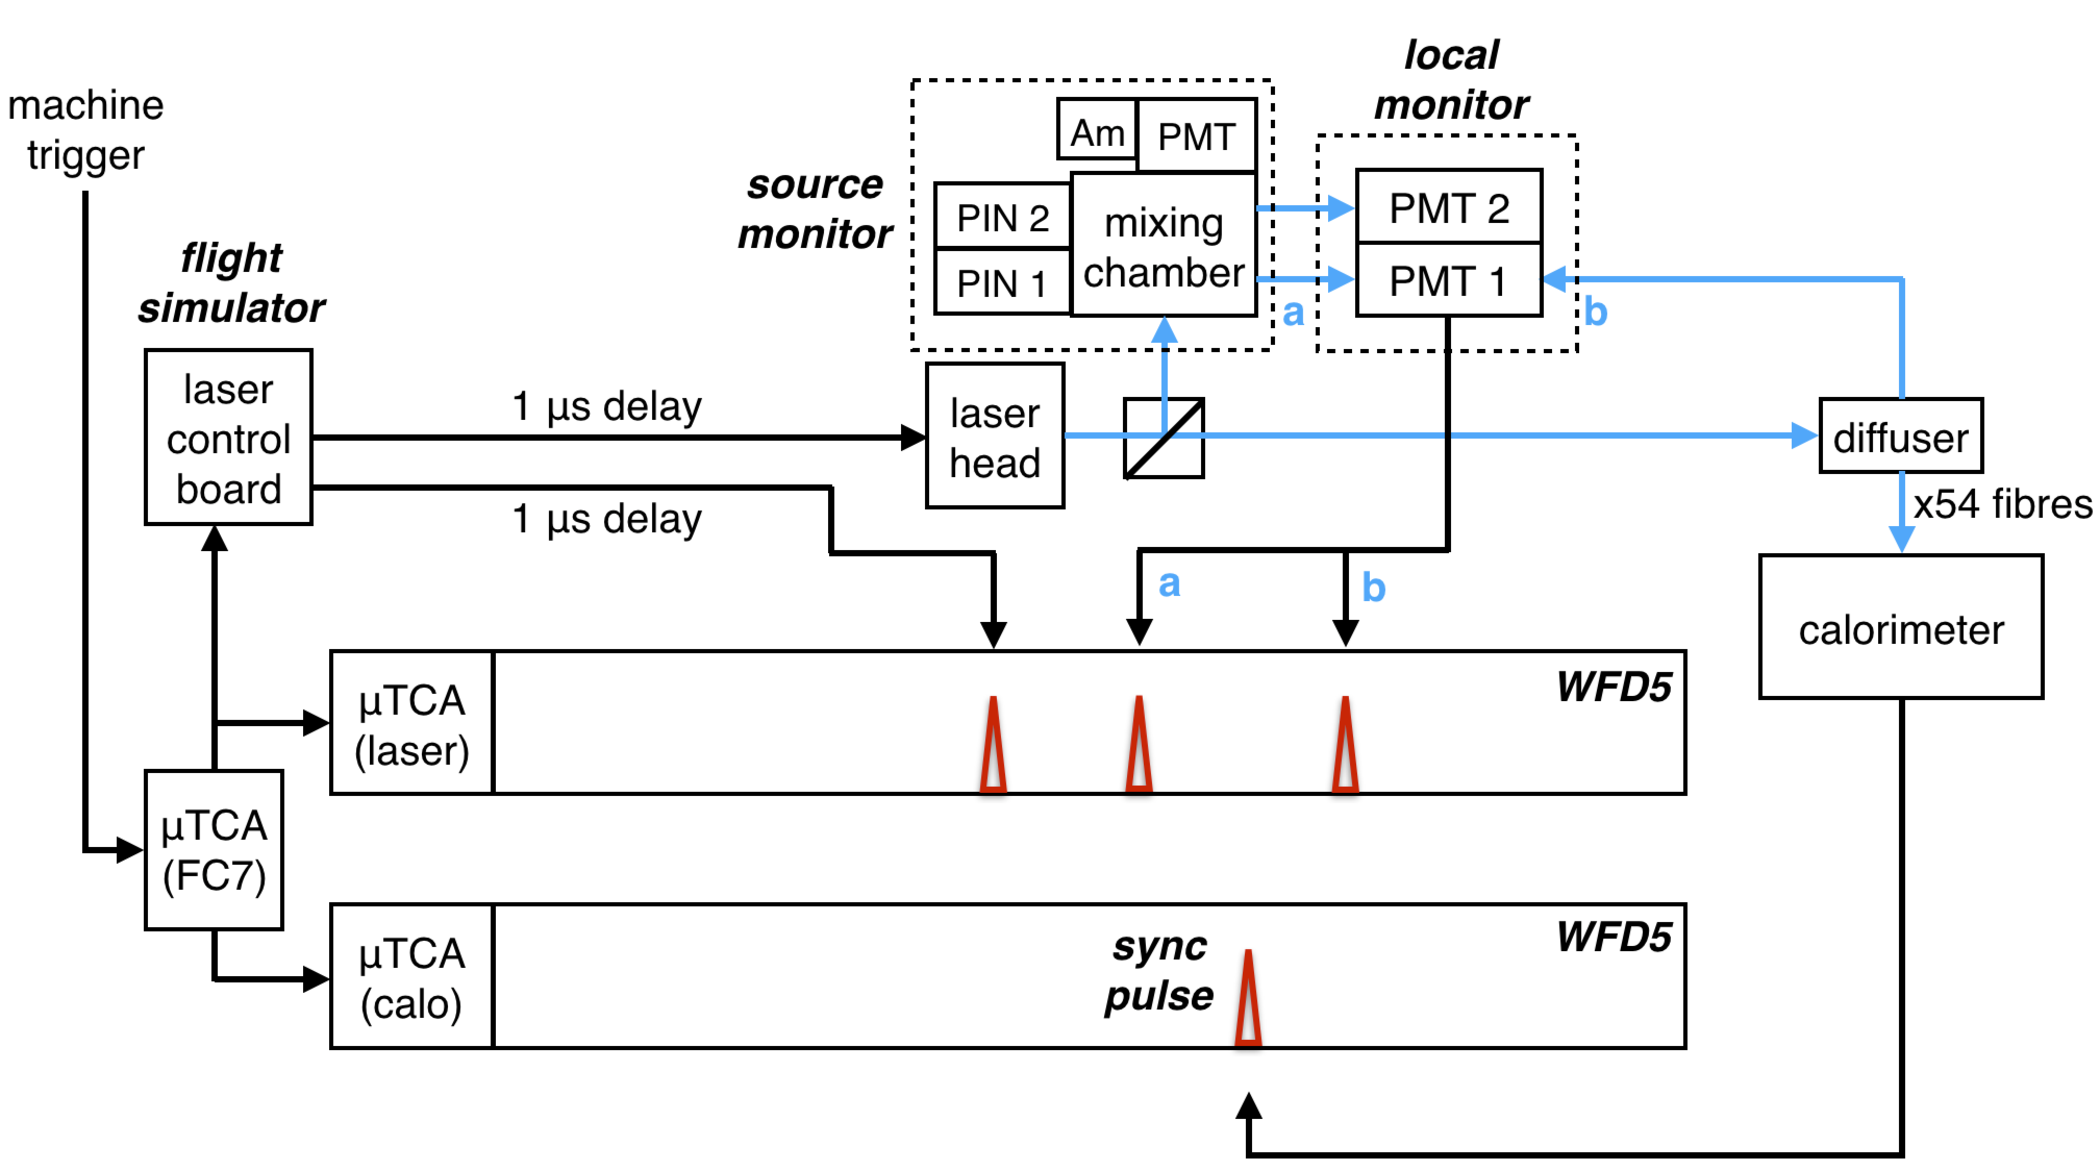
\includegraphics[width=0.75\textwidth]{pics/TimingPropagation.pdf} 
%\caption{Simplified diagram for the timing propagation in the calorimetry system. This is %specific for the SLAC test beam but will be very similar for the Muon g-2 experiment.}%\label{fig:TimingPropagation}
%\end{figure}

To understand who these signals can be used for time alignment, let us look at the general timing propagation in the calorimetry and laser system at the SLAC test beam shown in Fig.~\ref{fig:SyncTime} and Fig.~\ref{fig:BeamTime}. 

\subsection{Sync pulse}

\begin{figure}[htbp]
\centering
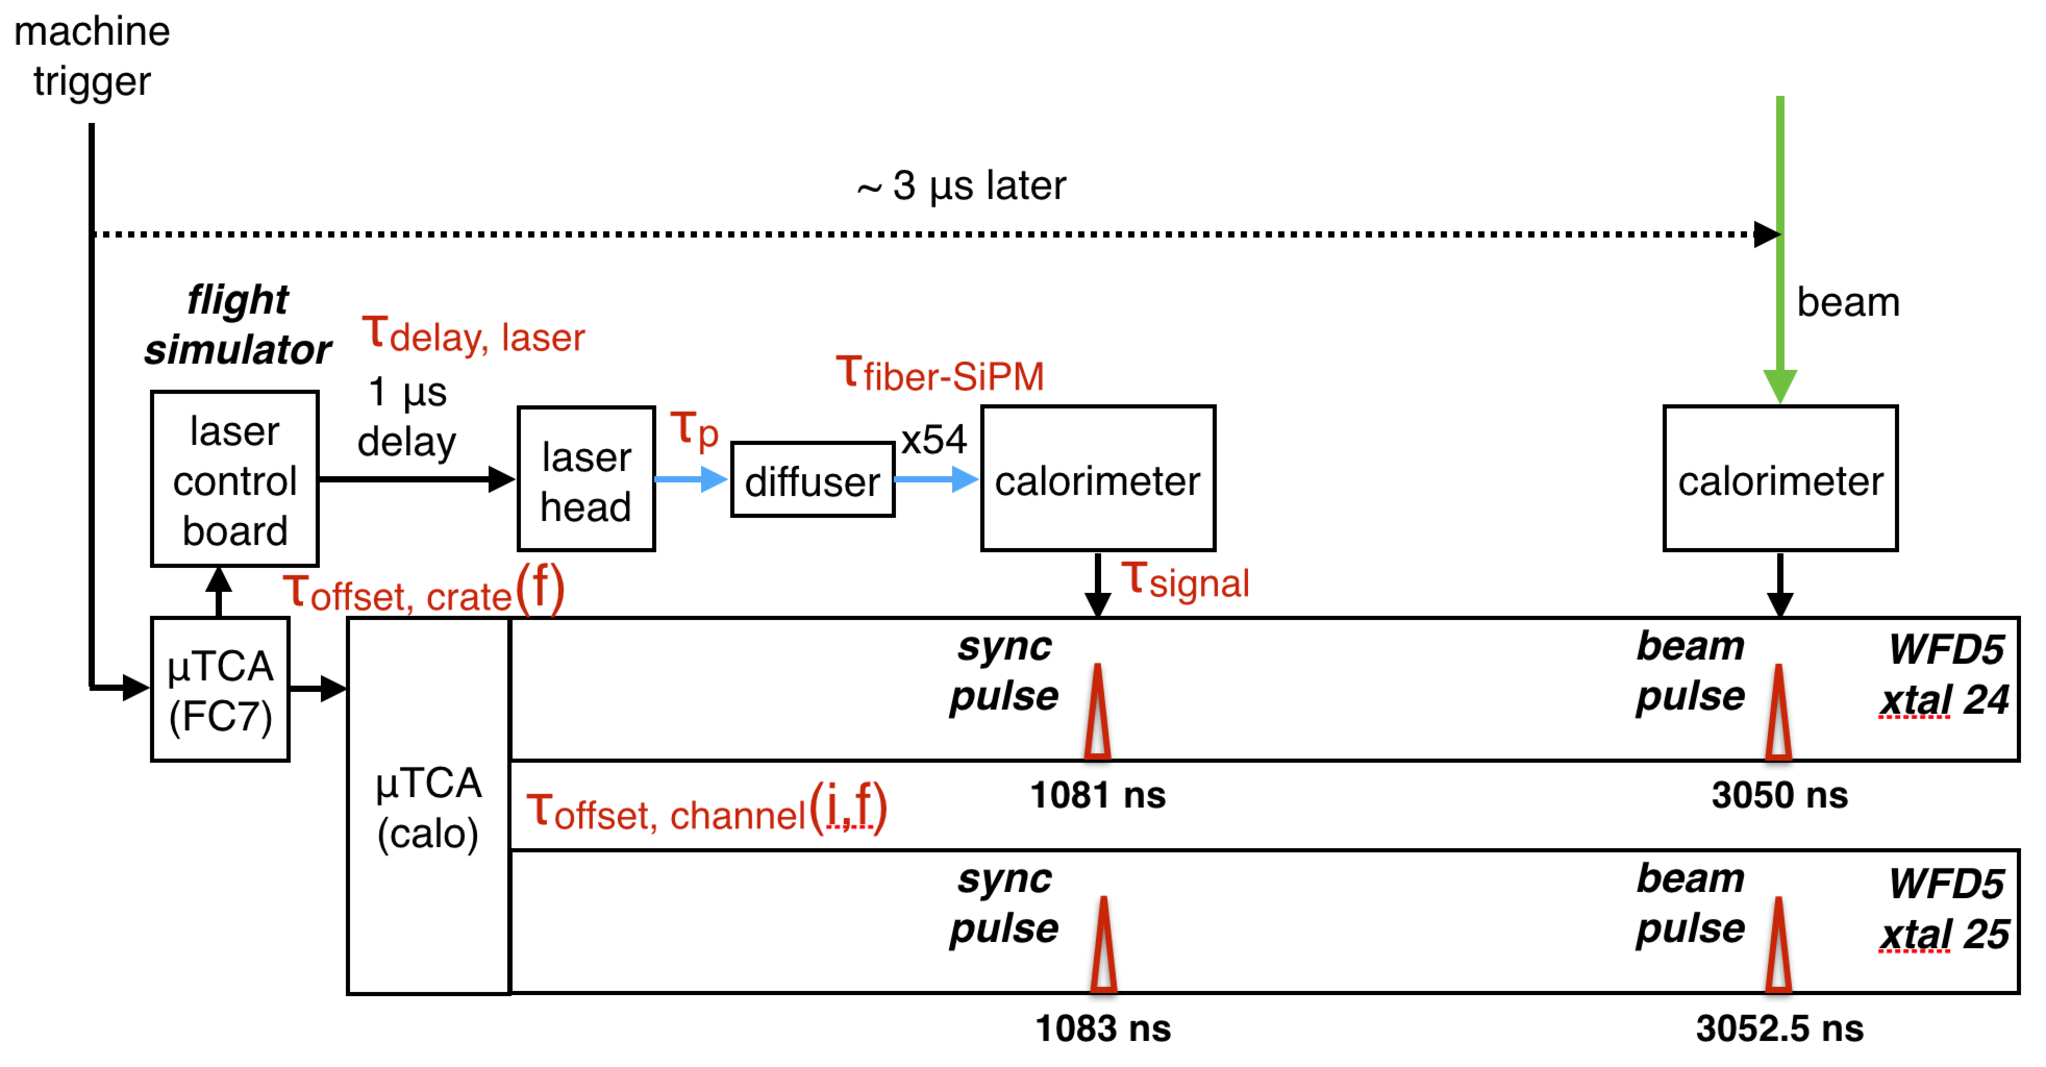
\includegraphics[width=0.7\textwidth]{pics/SyncTimeFormulation.pdf} 
\caption{A diagram depicting timing information related to the formulation of the laser sync pulse time, $t_{sync}(f,i)$.}\label{fig:SyncTime}
\end{figure}

Based on Fig.~\ref{fig:SyncTime}, the time extracted from the template fit of a sync pulse for crystal $i$ and fill $f$ can be written as
%
\begin{equation}
t_{sync}(f,i) = [ \tau_{\rm{delay,laser}} - \tau_{\rm{offset,board}}(f) - \tau_{\rm{offset,channel}}(f,i) ]  + \tau_{\rm{p}} + \tau_{\rm{fiber}}(i) + \tau_{\rm{signal}} \label{eq:tsync}
\end{equation}
%
where $\tau_{delay,laser}$ is the delay of the laser pulse trigger set in the laser control board, $\tau_{\rm{offset,board}}(f)$ is the time offset of the laser control board trigger (before delay) relative to the trigger received from the FC7, $\tau_{\rm{offset,channel}}(f)$ is the WFD5's trigger signal relative to the trigger received from the $\mu$TCA crate, $\tau_{\rm{p}}$ is the propagation time from the laser head to the diffuser inside the calorimeter box, $\tau_{\rm{fiber}}(i)$ is the time taken by the light to reach the SiPM $i$ from the fiber bundle attached to the diffuser, and $\tau_{\rm{signal}}$ is the propagation time of the signal from the SiPM to the channel in WFD5.

\subsection{Beam pulse}

\begin{figure}[htbp]
\centering
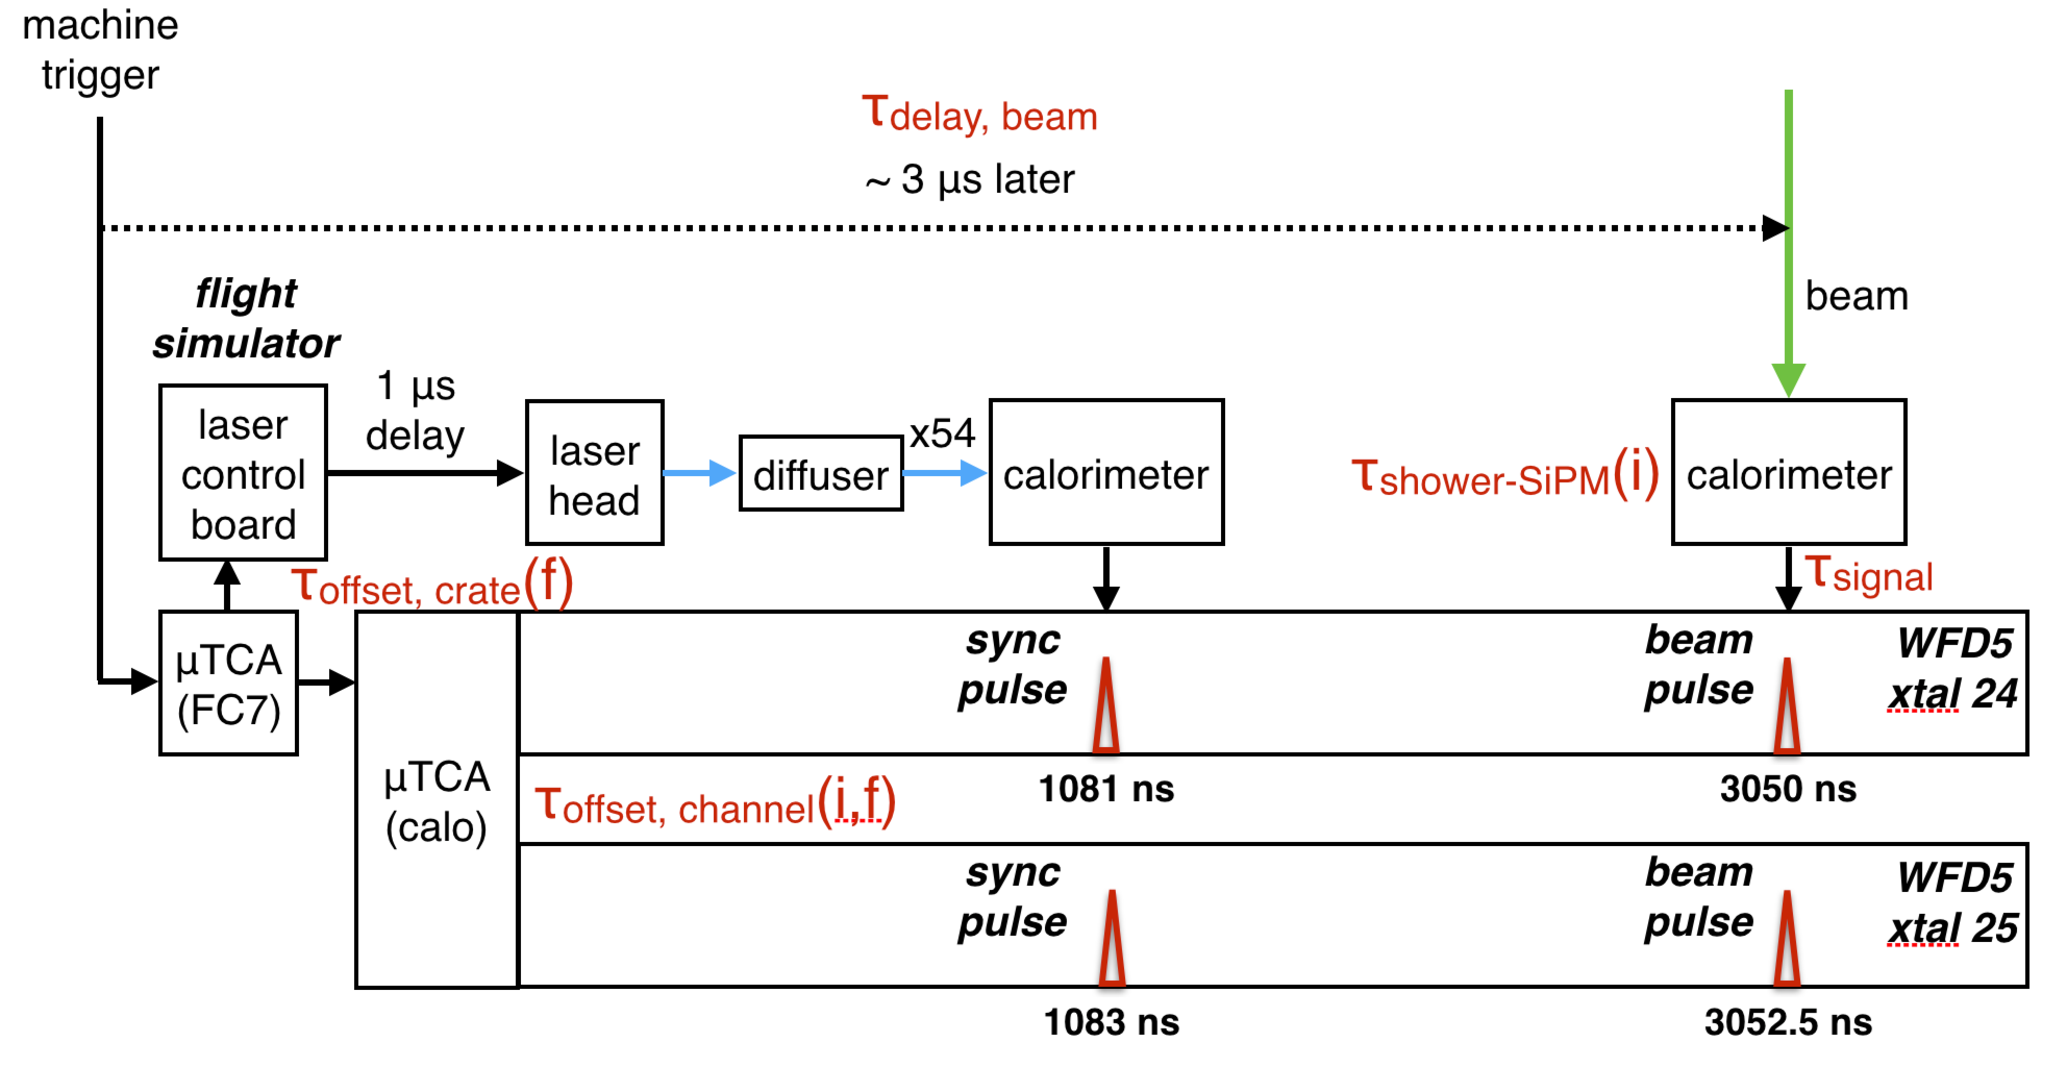
\includegraphics[width=0.7\textwidth]{pics/BeamTimeFormulation.pdf} 
\caption{A diagram depicting timing information related to the formulation of the beam pulse time, $t_{beam}(f,i)$.}\label{fig:BeamTime}
\end{figure}

Likewise, for an electron/positron beam in Fig.~\ref{fig:BeamTime},
%
\begin{equation}
t_{beam}(f,i) = [\tau_{\rm{delay,beam}}(f) - \tau_{\rm{offset,crate}}(f) - \tau_{\rm{offset,channel}}(f,i) ]  + \tau_{\rm{shower}}(i) + \tau_{\rm{signal}} \label{eq:tbeam}
\end{equation}
%
where $\tau_{\rm{delay,beam}}(f)$ is the delay of the electron beam relative to the time the FC7 receives trigger, $\tau_{\rm{offset,crate}}(f)$ is the offset between the machine trigger at the trigger in the calorimeter $\mu$TCA crate, $\tau_{\rm{shower}}(i)$ is the shower propagation time of the beam to the SiPM $i$.

\subsection{Cosmic pulse}

Similarly, for a cosmic ray (just replace beam with cosmic),
%
\begin{equation}
t_{cosmic}(f,i) = [\tau_{\rm{delay,cosmic}}(f) - \tau_{\rm{offset,crate}}(f) - \tau_{\rm{offset,channel}}(f,i) ]  + \tau_{\rm{cosmic}}(i) + \tau_{\rm{signal}} \label{eq:tcosmic}
\end{equation}
%
where $\tau_{\rm{delay,cosmic}}$ is the delay of the cosmic beam relative to the machine trigger, $\tau_{\rm{cosmic}}(i)$ is the shower propagation time of the cosmic beam shower to the SiPM $i$.

\subsection{Time distribution for sync and beam pulses}

Time distribution for the sync and beam pulses are shown in Fig.~\ref{fig:DiffTiming_run1936}.
The widths of first two distributions are about 25 ns and 10 ns. These numbers correspond very well with the dependence of these times on $\tau_{\rm{offset,board}}(f)$ and $\tau_{\rm{offset,crate}}(f)$ terms which are the uncertainties on the 40 MHz (CCC system) and 100 MHz (laser control board) clocks. Since these two clocks are not synchronized to each other, the difference between the two times have a broader distribution as shown in Fig.~\ref{fig:DiffTiming_run1936}(right).

\begin{figure}[htbp]
\centering
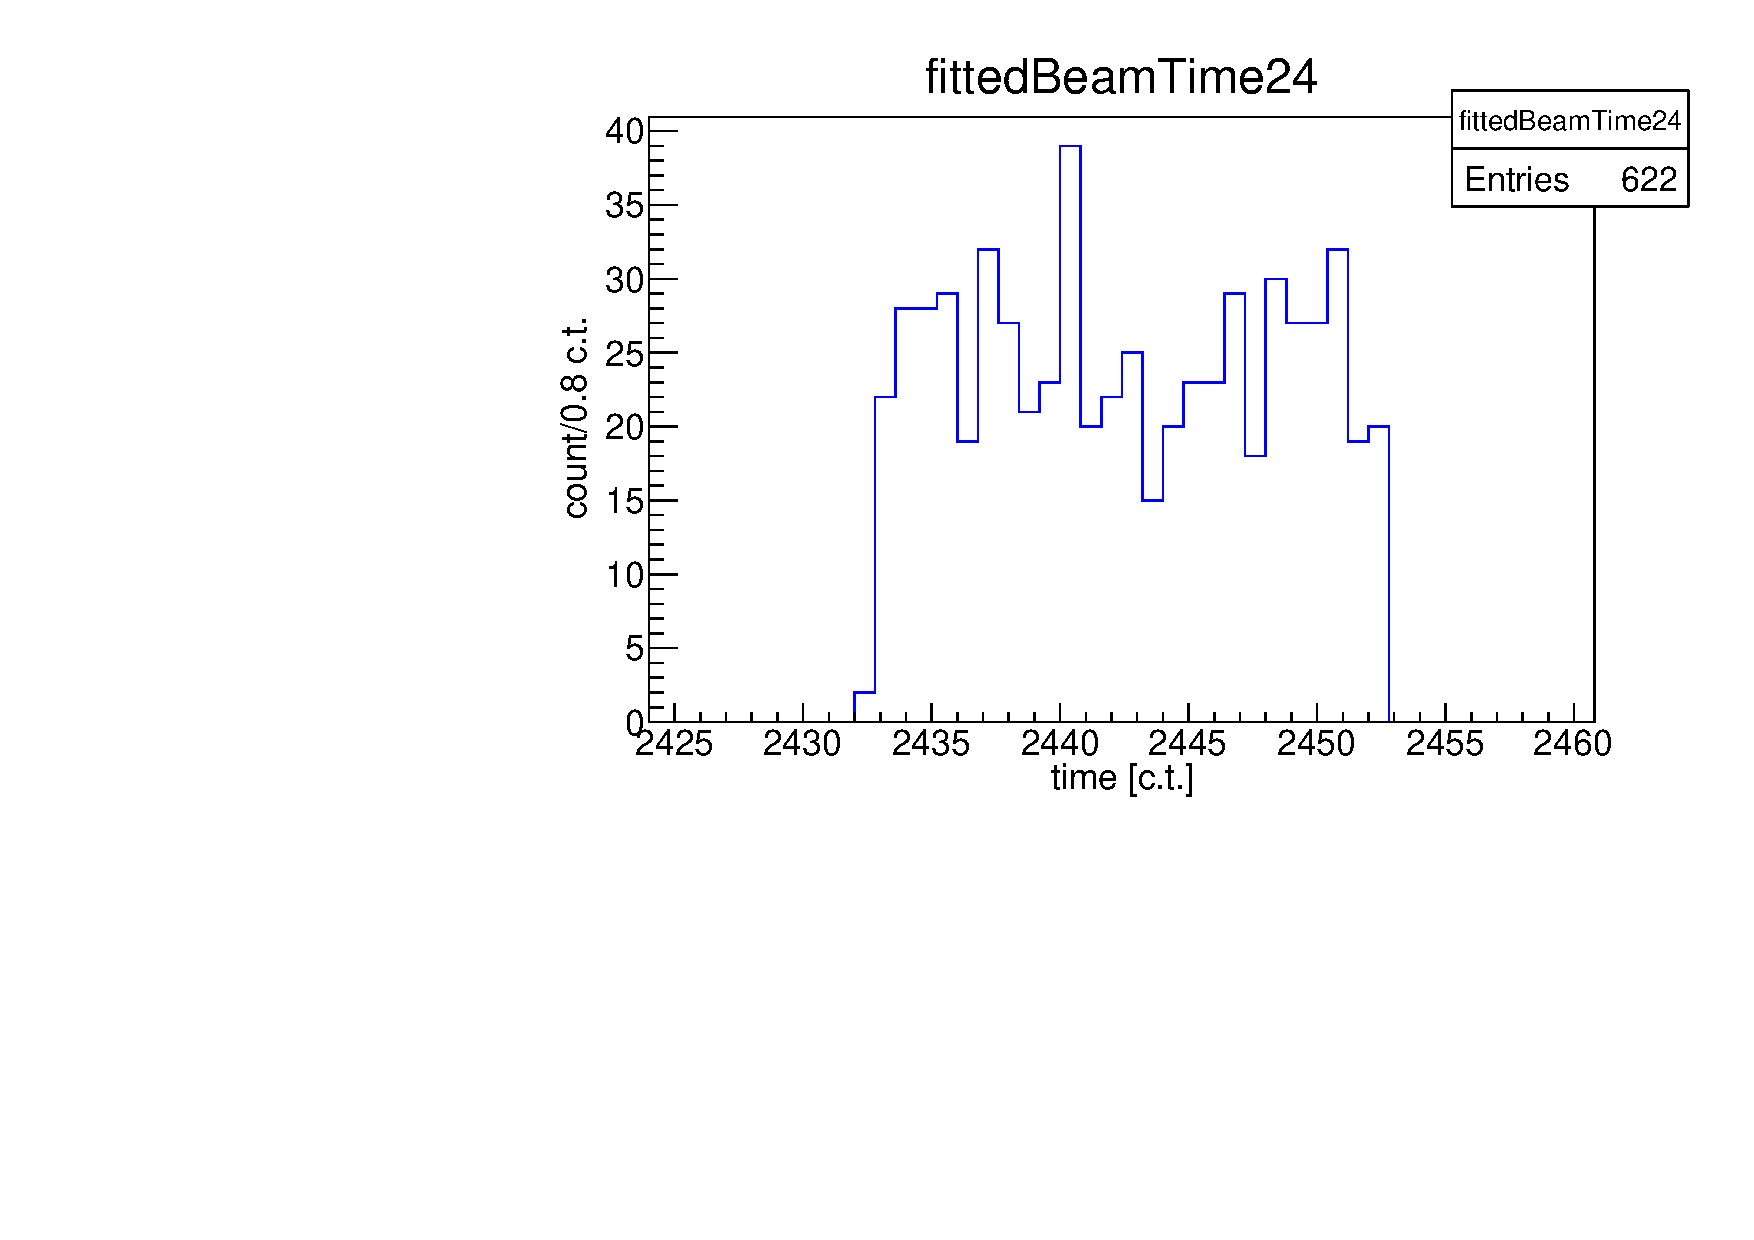
\includegraphics[width=0.31\textwidth]{pics/fittedBeamTime24_run1935.pdf} 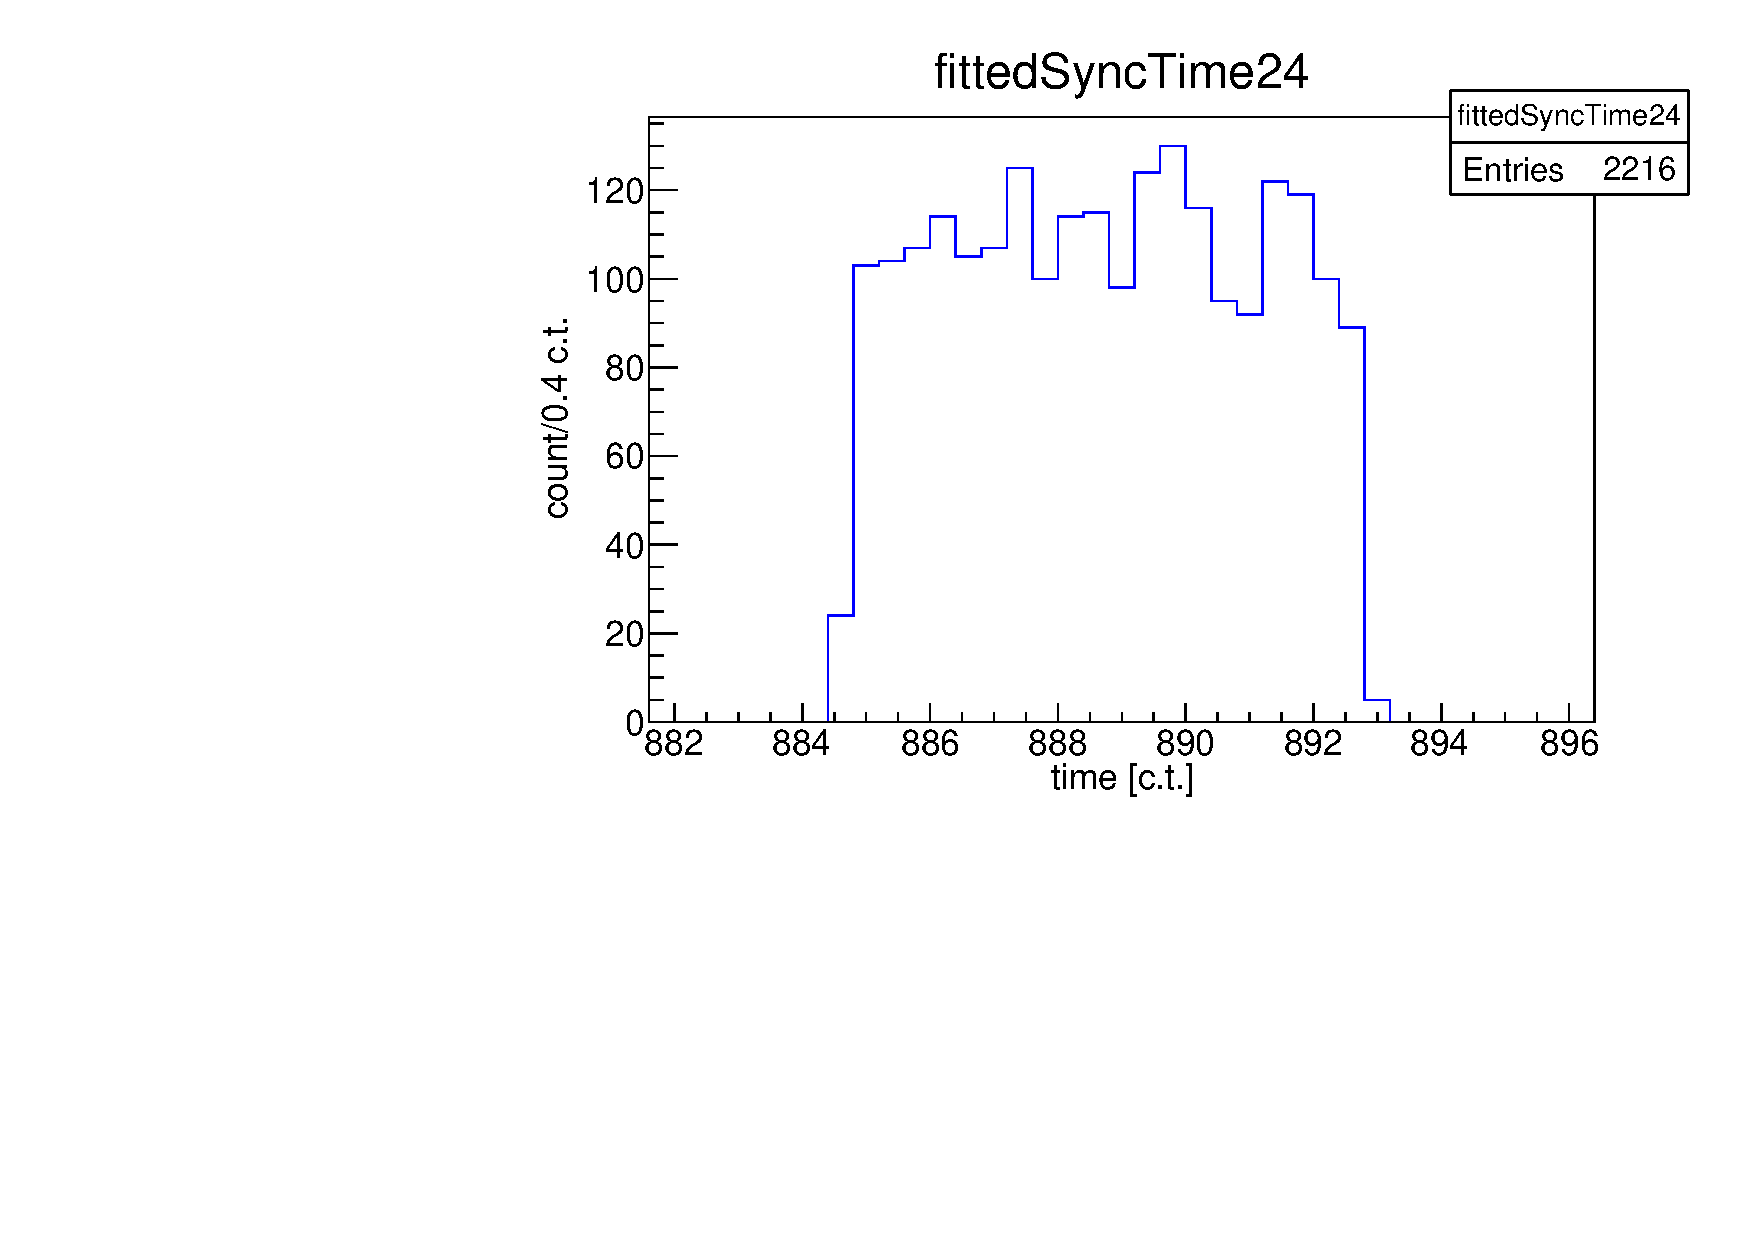
\includegraphics[width=0.31\textwidth]{pics/fittedSyncTime24.pdf} 
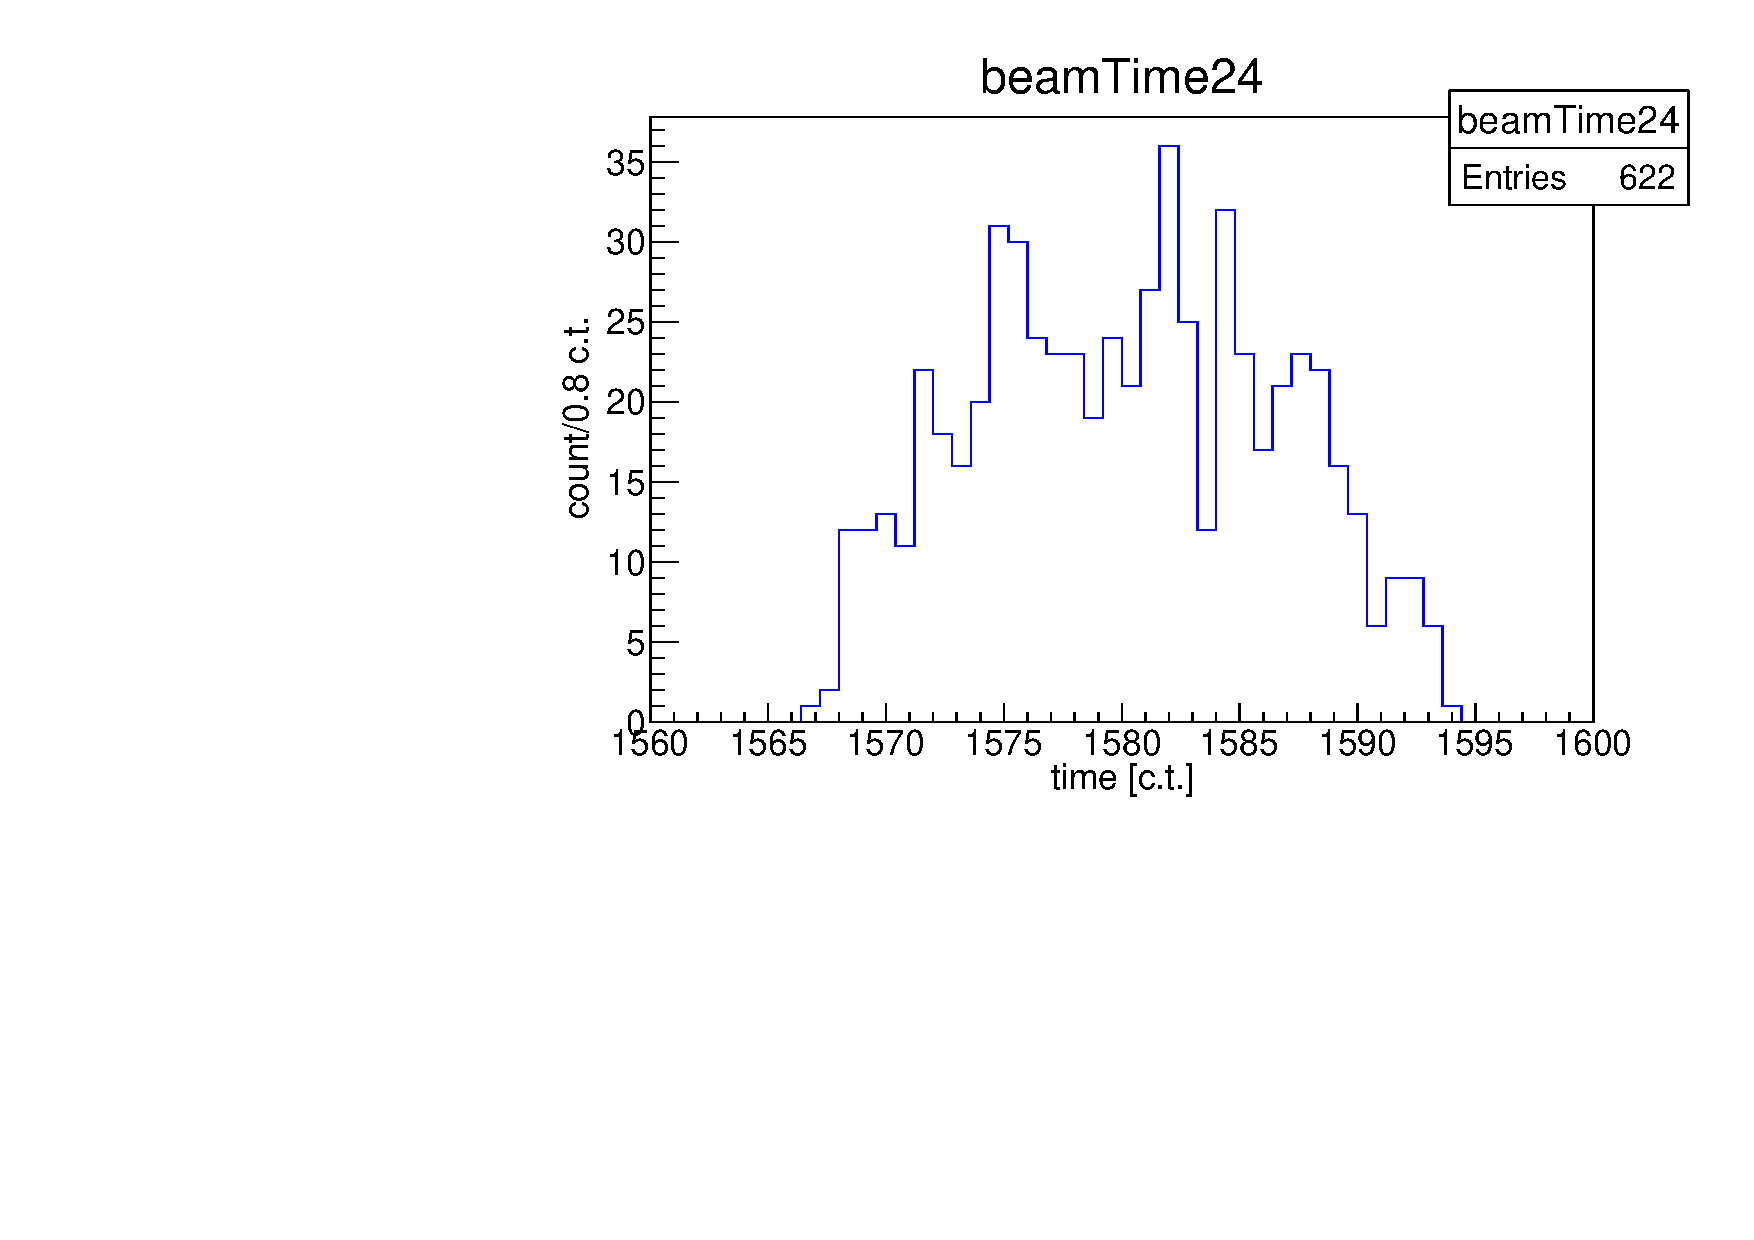
\includegraphics[width=0.31\textwidth]{pics/beamTime24_run1935.pdf} 
\caption{Distribution of (left) fitted beam time, (middle) fitted sync pulse time, and (right) synced beam time from the SLAC test beam 2016, run number 1935.}\label{fig:Timing_run1935}
\end{figure}

\section{Time alignment}

To demonstrate why a dedicated time alignment procedure is needed, let us look at the time difference between two channels, $i$ and $j$. The beam time difference $dt_{beam}(f,i,j)$ is given by
%
\begin{equation}
dt_{beam}(f,i,j) = d\tau_{\rm{offset,channel}}(f,i,j)  + d\tau_{\rm{shower}}(i,j) \label{eq:dtbeam}
\end{equation}
%
and it is very clear that we need to take the offset between WFD5 channels -- $d\tau_{\rm{offset,channel}}(f,i,j)$ into account if we want to get an unbiased measurement of $d\tau_{\rm{shower}}(i,j)$. Similarly, if we look at the cosmic events, we get
%
\begin{equation}
dt_{cosmic}(f,i,j) = d\tau_{\rm{offset,channel}}(f,i,j)  + d\tau_{\rm{cosmic}}(i,j)~. \label{eq:dtcosmic}
\end{equation}
%

On the other hand, the sync time difference $dt_{sync}(f,i,j)$ between channel $i$ and $j$ is given by
%
\begin{equation}
dt_{sync}(f,i,j) = d\tau_{\rm{offset,channel}}(f,i,j) + d\tau_{\rm{fiber}}(i,j)
\label{eq:dtsync}
\end{equation}
%
and the \textit{synced beam time} difference $dt_{sbeam}(f,i,j)$ is given by
%
\begin{equation}
dt_{sbeam}(i,j) = dt_{beam}(f,i,j) - dt_{sync}(f,i,j) = d\tau_{\rm{shower}}(i,j) - d\tau_{\rm{fiber}}(i,j)
\label{eq:dtsbeam}
\end{equation}

Obviously, since the sync laser pulses are delivered by the fiber bundle, there is a dependency on the difference in the fiber propagation time, $ d\tau_{\rm{fiber}}(i,j)$ .
Among the four terms on the right hand sides of Eq.~\ref{eq:dtbeam}, \ref{eq:dtcosmic} and \ref{eq:dtsync}, $d\tau_{\rm{shower}}(i,j)$ and $d\tau_{\rm{cosmic}}(i,j)$ depend on the kinematics of the particle involved. $d\tau_{\rm{offset,channel}}(f,i,j)$ is pretty stable unless there is any initialization of the WFD5 and $d\tau_{\rm{fiber}}(i,j)$ is basically constant.

Distribution of the time difference between crystal 15th and crystal 33th for an electron event and a sync pulse event is shown in Fig.~\ref{fig:DiffTiming_run1936}.
\begin{figure}[htbp]
\centering
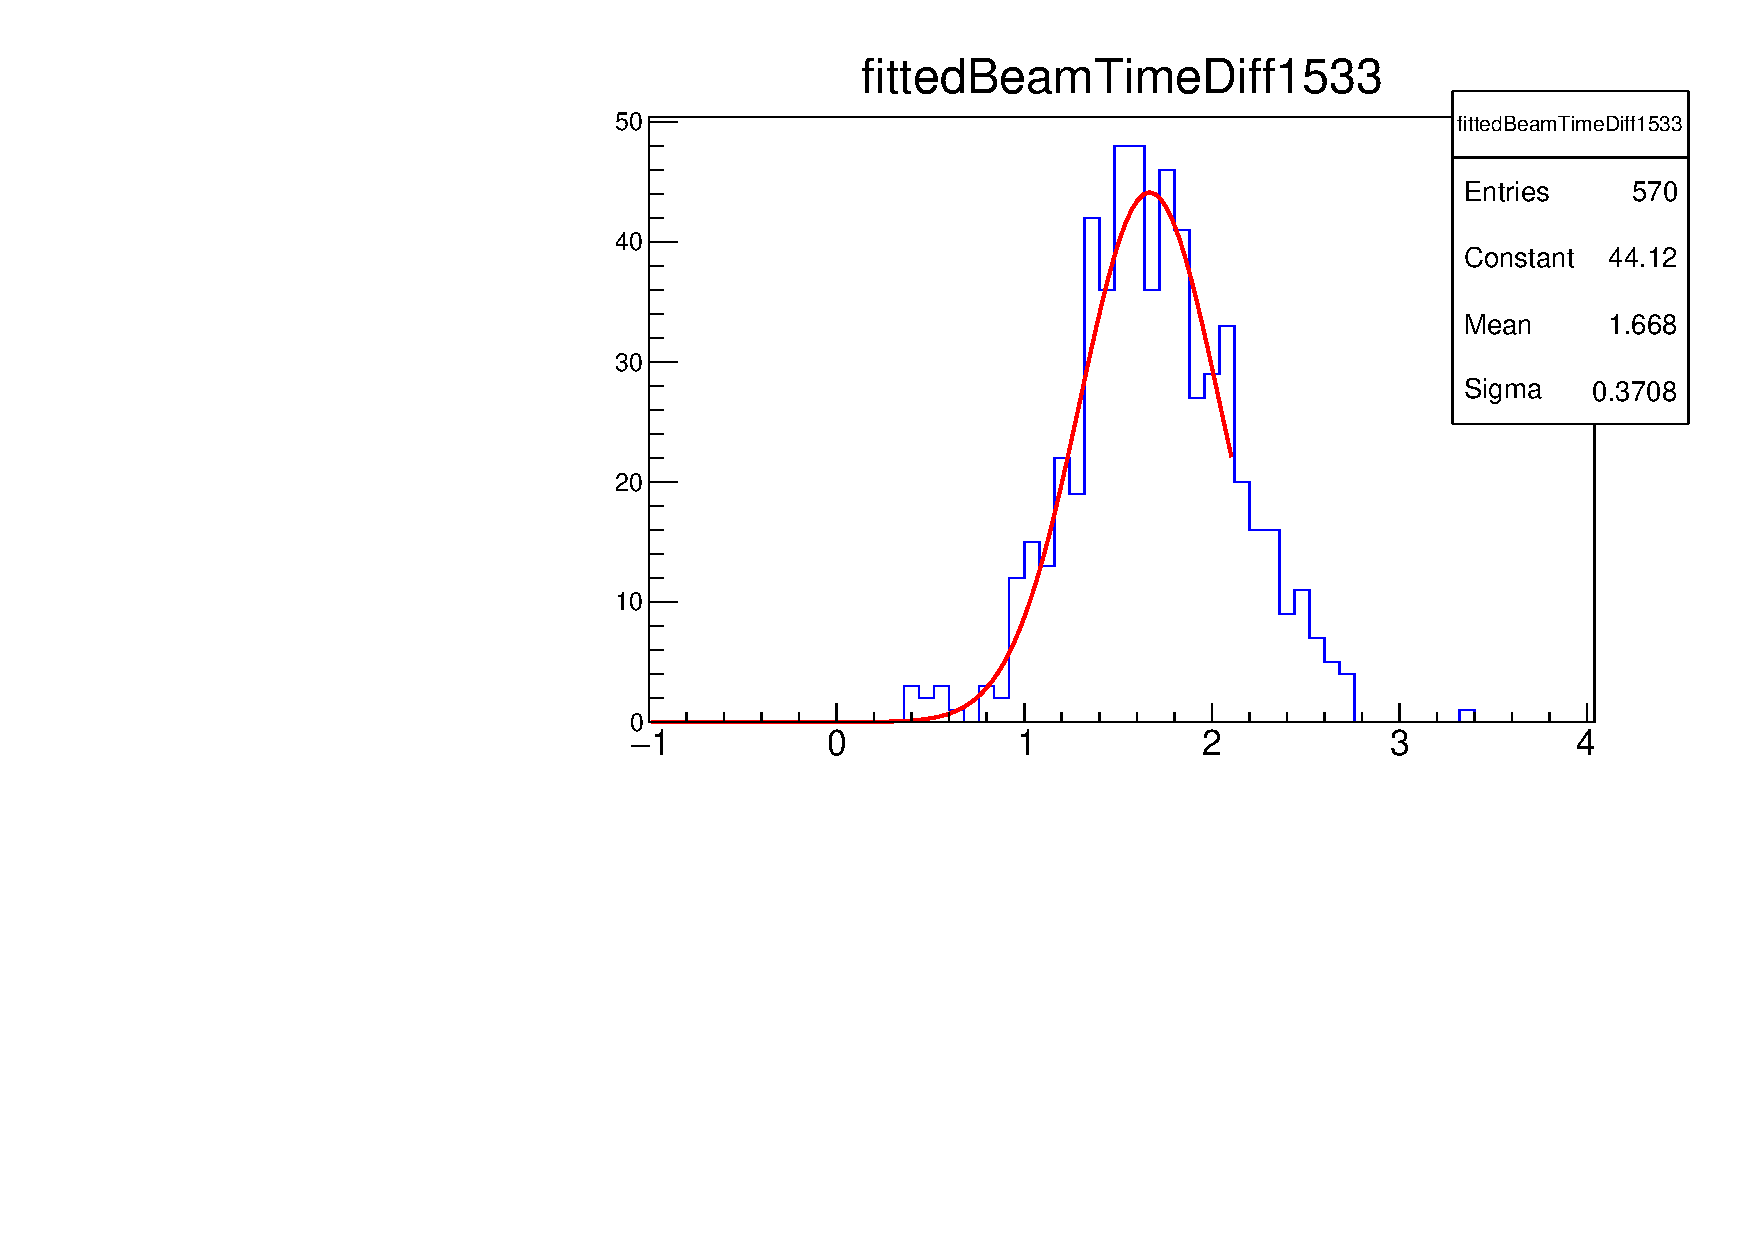
\includegraphics[width=0.31\textwidth]{pics/fittedBeamTimeDiff1533.pdf} 
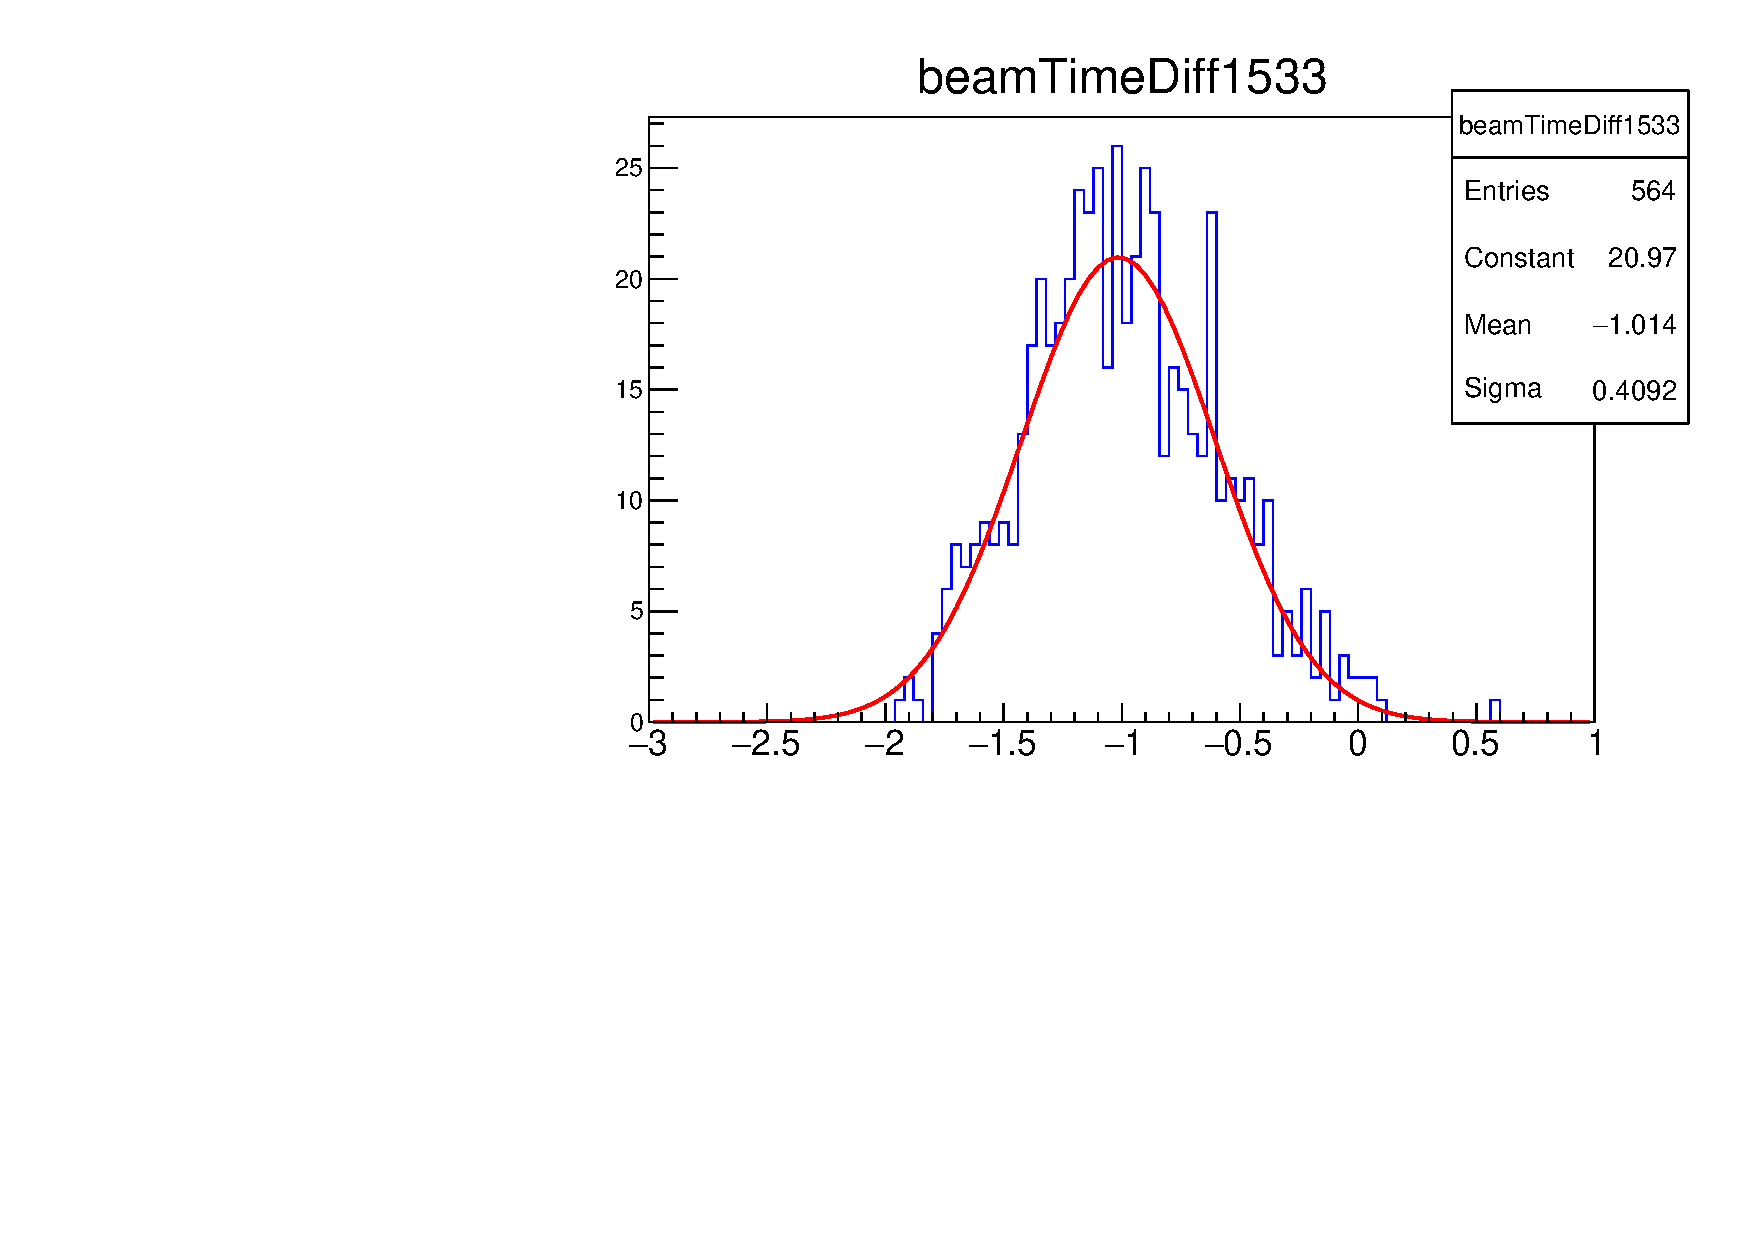
\includegraphics[width=0.31\textwidth]{pics/beamTimeDiff1533.pdf} 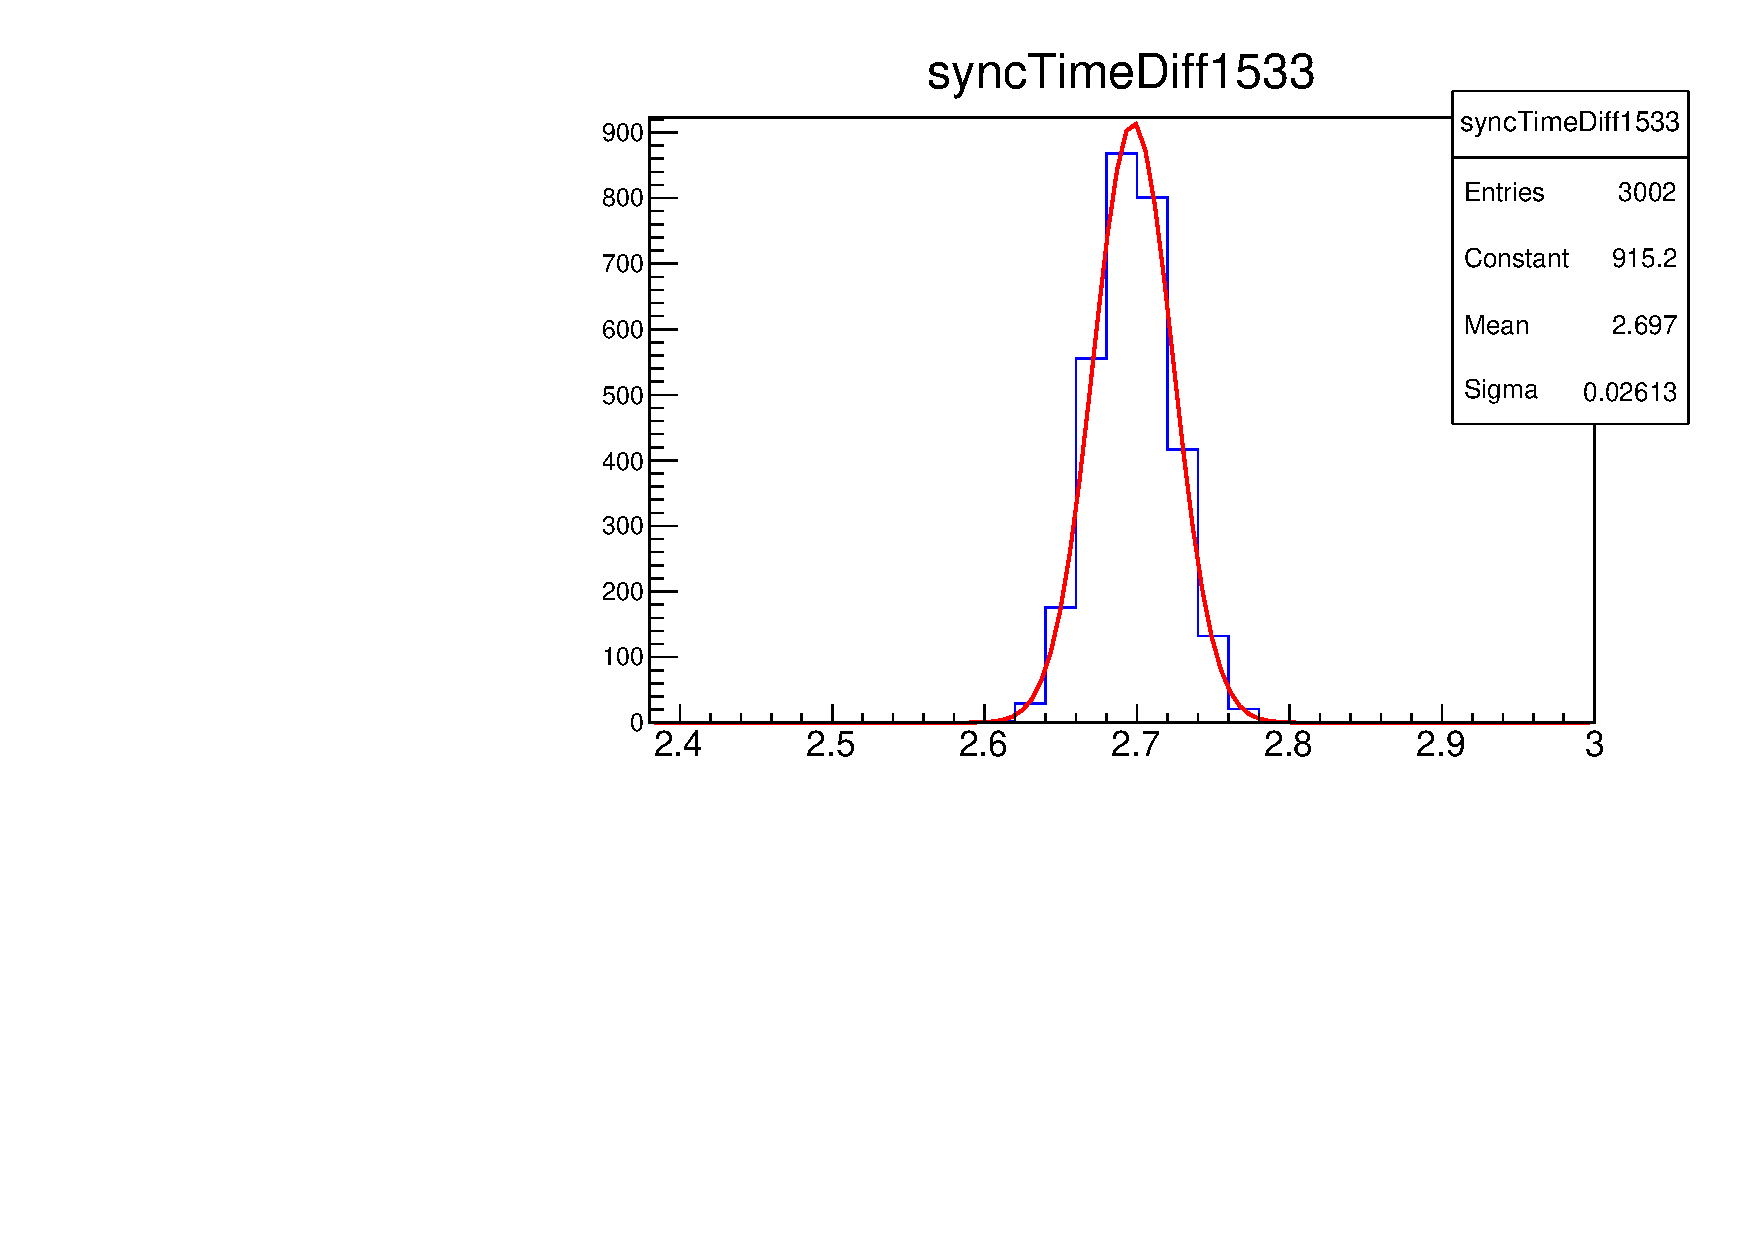
\includegraphics[width=0.31\textwidth]{pics/syncTimeDiff1533.pdf}
\caption{Distribution of (left) fitted beam time difference and (middle) synced beam time difference, and (right) sync time difference from the SLAC test beam 2016, run number 1936.}\label{fig:DiffTiming_run1936}
\end{figure}

Hence we need to find a way to extract the propagation time in the fiber, $t_{\rm{fiber-SiPM}}$, for all 54 fibers. Bad news is, it is not trivia to measure each fiber's propagation time up to 100~ps precision. Good news is, we just need to measure the relative difference within a calorimeter. For historical reason,
we have selected the crystal 24's rider channel as the reference point.

\subsection*{Alignment using sync pulse and beam pulse}

Aligning all the timing information w.r.t to the crystal 24, we have

\begin{align}
\delta t_{sync}(i,24,f)   &= t_{sync}(f,i) - t_{sync}(24,f)  \\
                         &= \left[\tau_{fiber}(i) -  \tau_{fiber}(24) \right]+ \left[\tau_{rider}(f,i) -  \tau_{rider}(24,f) \right] \\
                         &= \delta \tau_{fiber}(i,24) + \delta \tau_{rider}(i,24,f) \label{eq:tsync24}
\end{align}
%
and
%
\begin{align}
\delta t_{beam}(i,24,f)  &= t_{beam}(f,i) - t_{beam}(24,f)  \\
                         &= \left[ \tau_{shower}(f,i) -  \tau_{shower}(24,f)  \right] + \left[ \tau_{rider}(f,i) -  \tau_{rider}(24,f) \right] \\
                         &= \delta \tau_{shower}(i,24,f) + \delta \tau_{rider}(i,24,f)~.\label{eq:tbeam24}
\end{align}

If we choose all the events such that the shower propagation time in the crystal is the same w.r.t. to the crystal 24, i.e. $\delta \tau_{shower}(i,24,f)=0$ (for example, beam hitting the center of the crystal or hitting at the common border of the crystals),
then we have
%
\begin{equation}
\delta t_{beam}(i,24,f)   = \delta \tau_{rider}(i,24,f)~.
\end{equation}
%
Since the offset in the rider $\tau_{rider}$ is the same for all the fills within the same run, 
%
\begin{equation}
\delta t_{beam}(i,24)   = \delta \tau_{rider}(i,24)~.
\end{equation}
%
Of course, since the shower is well contained within the $3\times3$ crystals, it is not possible to map out all the $\delta \tau_{rider}$ by just analyzing
the data w.r.t. to the crystal 24. Hence to have a complete map, we need to look at the $\delta \tau_{rider}$ w.r.t. to the crystals that have the  $\delta \tau_{rider}$ extracted compared to crystal 24. The statistical uncertain will increase but there should be an optimum way of doing it out there.

\subsection*{Symmetry shower shape}

We can use the fact that the EM shower shape is symmetry on average. Arrival time should be the same on average for crystals with similar energy. Three different topologies can be used and are shown in Fig.~\ref{fig:ShowerTopology}.

\begin{figure}[htbp]
\centering
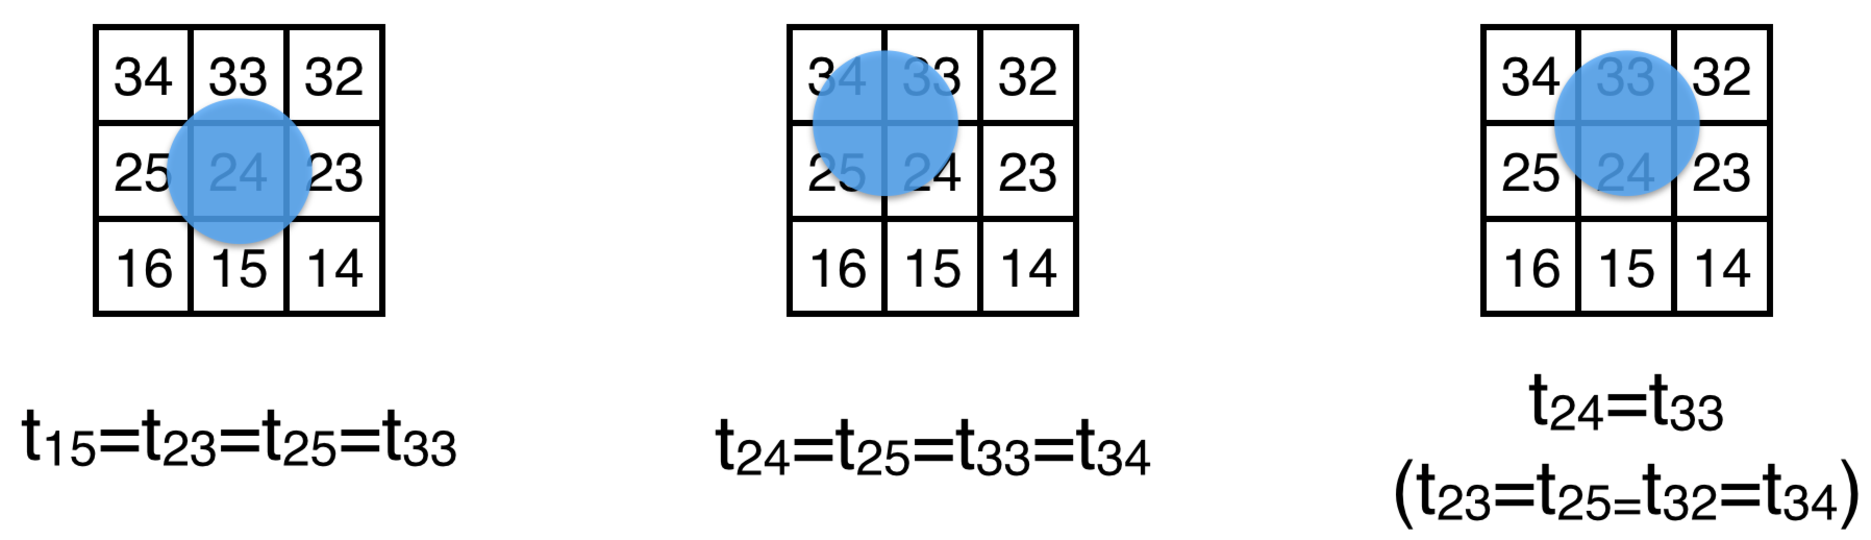
\includegraphics[width=0.75\textwidth]{pics/ShowerTopology.pdf} 
\caption{Three different types of shower topology that can be used for the offset extraction.}\label{fig:ShowerTopology}
\end{figure}

An example of the $dt(i,24)$ distribution is shown in Fig.~\ref{fig:dti24Distribution}.
\begin{figure}[htbp]
\centering
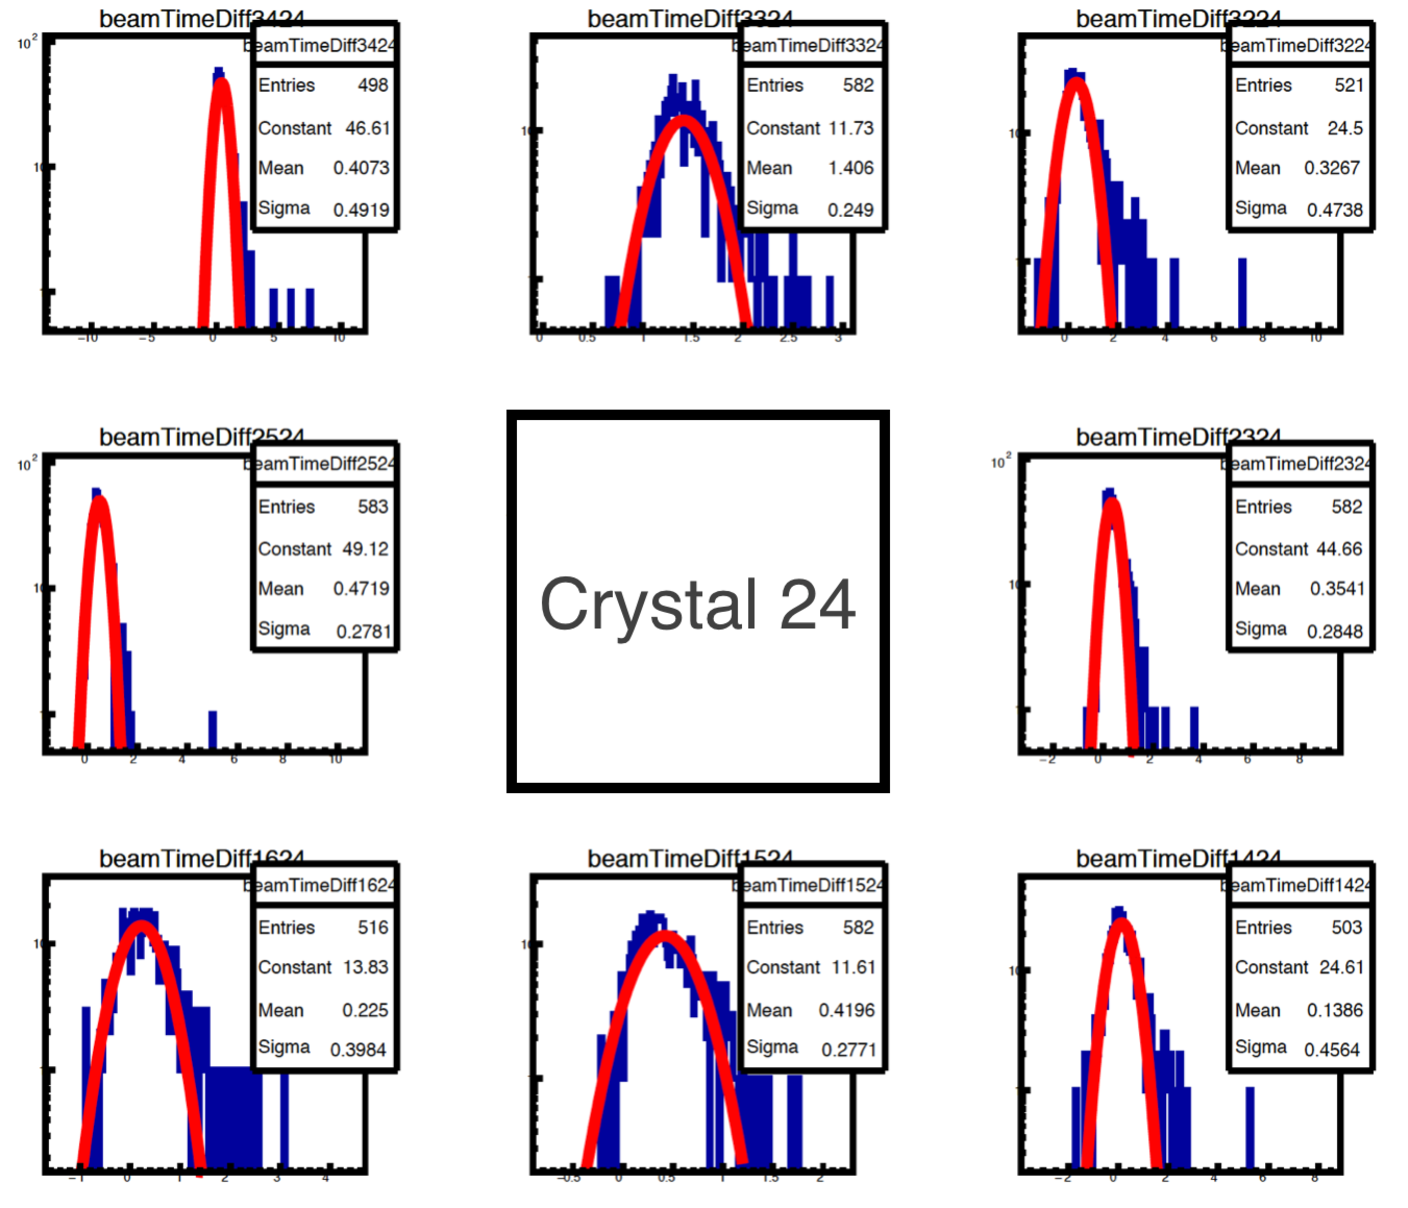
\includegraphics[width=0.6\textwidth]{pics/dt_i_24_Distribution.pdf} 
\caption{An example of the $dt(i,24)$ distribution.}\label{fig:dti24Distribution}
\end{figure}

\begin{figure}[htbp]
\centering
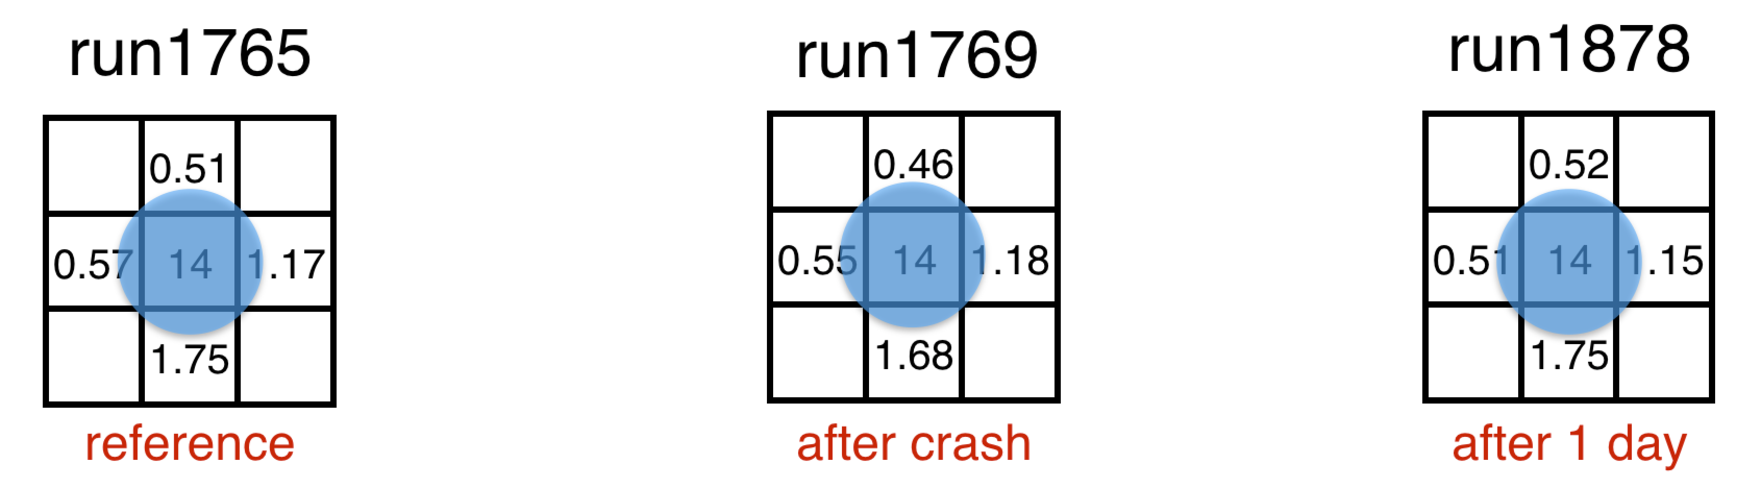
\includegraphics[width=0.75\textwidth]{pics/dt_fiber_Stability.pdf} 
\caption{Stability of the extraction of $\delta t_{\rm{fiber-SiPM}}$. The values remain within each after a DAQ crash or after one day of DAQ running, implying that it is really the fiber length offsets we are measuring.}\label{fig:dtFiberStability}
\end{figure}

Once we have the map of the $\delta \tau_{\rm{rider}}$, we can solve Eq.~\ref{eq:tsync24} and get $\delta \tau_{\rm{fiber}}$.

\begin{figure}[htbp]
\centering
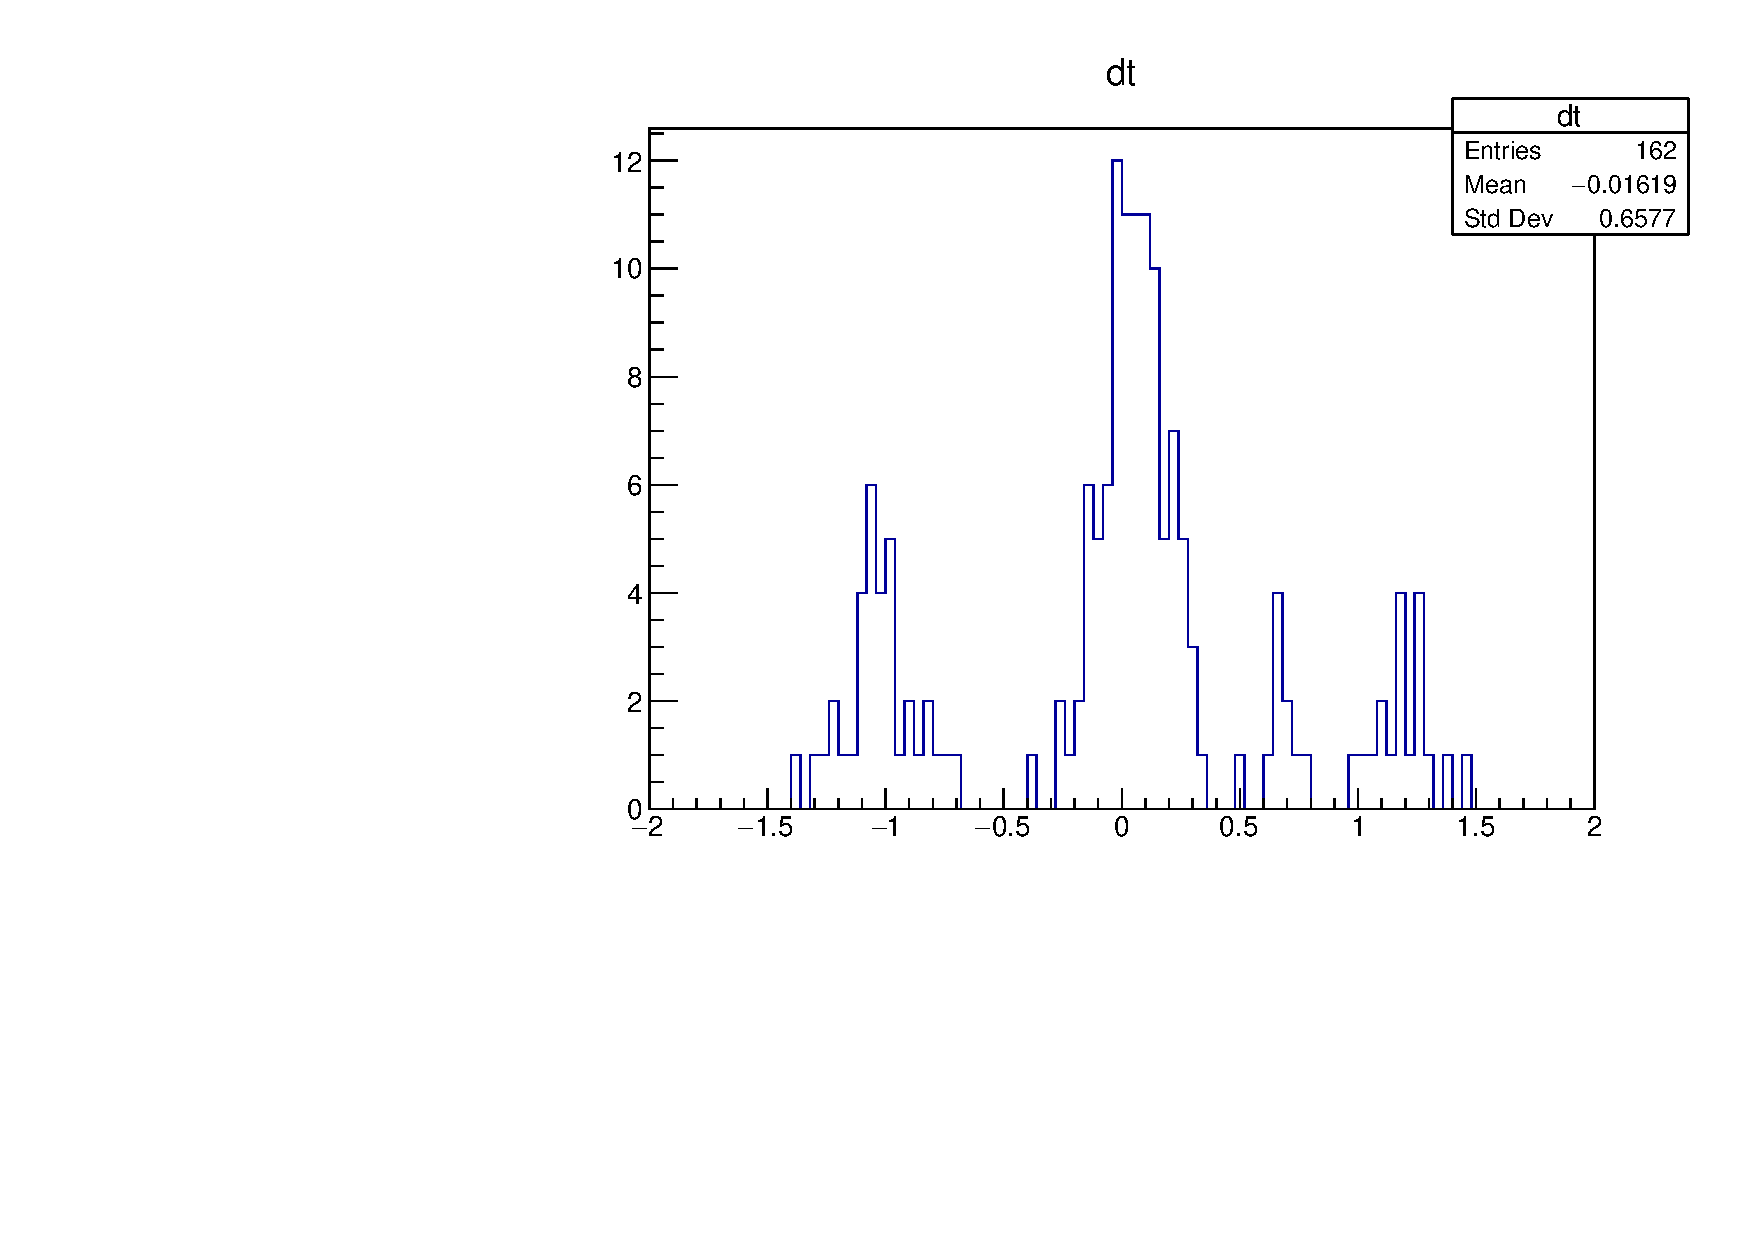
\includegraphics[width=0.5\textwidth]{pics/grid.pdf} 
\caption{Distribution of $\delta t_{\rm{fiber-SiPM}}$}\label{fig:grid}
\end{figure}

If we turn things around, since we have all the $\delta \tau$ relative to crystal 24, we can also say that we have all the $\delta \tau$
relative to each other.

Going back to Eq.~\ref{eq:dtsbeam}, since we have the $\delta \tau_{fiber}$, we now have a better knowledge 
regarding $\tau_{shower}$. We can now discriminate more pile up events with this additional information.
We might also be able to disentangle the position and the angle information.



\section{Datasets}

\begin{table}[htbp]
\centering
\caption{Run list for 54 crystals.}
\begin{tabular}{|c|c|c|c|c|c|c|c|c|c|}
\hline 
\#    & col 9 & col 8 & col 7 & col 6 & col 5 & col 4 & col 3 & col 2 & col 1 \\
\hline
row 1 & 3284  & 3285  & 3286  & 3287  & 3288  & 3289  & 3292  & 3293  & 3294  \\
\hline
row 2 & 3283  & 3281  & 3278  & 3277  & 3276  & 3275  & 3274  & 3272  & 3268  \\
\hline
row 3 & 3253  & 3254  & 3256  & 3257  & 3258  & 3263  & 3265  & 3266  & 3267  \\
\hline
row 4 & 3233  & 3234  & 3232  & 3235  & 3236  & 3237  & 3238  & 3229  & 3240  \\
\hline
row 5 & 3252  & 3251  & 3250  & 3249  & 3248  & 3247  & 3246  & 3245  & 3244  \\
\hline
row 6 & 3368  & 3303  & 3302  & 3301  & 3300  & 3369  & 3297  & 3296  & 3295 \\
\hline
\end{tabular} 
\label{tab:runlist}
\end{table}

\section{Software}
\begin{table}[htbp]
\centering
\caption{Run list for 54 crystals.}
\begin{tabular}{|c|c|}
\hline 
Repository & Branch \\
\hline
gm2ringsim & feature/SLAC2016 \\
\hline
gm2calo & feature/SLAC2016 \\
\hline
gm2dataproducts & feature/SLAC2016 \\
\hline
\end{tabular} 
\label{tab:software}
\end{table}


\begin{thebibliography}{99}

\bibitem{daq}
W. Gohn, \emph{Data Acquisition for the New Muon g-2 Experiment at Fermilab},
Journal of Physics: Conference Series 664 082014 (2015) 

\bibitem{rider}
A. Chapelian, \emph{Development of the electromagnetic calorimeter waveform digitizers for the Muon g-2 experiment at Fermilab},
PoS, EPS-HEP2015, 280 (2015)

\bibitem{fc7}
M. Pesaresi, et al., \emph{The FC7 AMC for generic DAQ \& control applications in CMS},
JINST 10, C03036 (2015)

\bibitem{amc13}
E. Hazen et al., \emph{The AMC13XG: a new generation clock/timing/DAQ module for CMS MicroTCA}
JINST 8, C12036 (2013)

\end{thebibliography}


\end{document}
